\chapter{ANALISIS DAN PERANCANGAN}
	
\section{\emph{Planning} (Perencanaan)}
Pada tahap \emph{planning} (perencanaan) ini yang pertama peneliti lakukan adalah mendefinisikan ruang lingkup dari penelitian ini. Kemudian melakukan analisis permasalahan terhadap sistem yang sedang berjalan dan juga menganalisis kebutuhan dari sistem yang akan dibangun.

	\subsection{Mendefinisikan Ruang Lingkup (\emph{Scope Definition})}
	Untuk lebih memfokuskan penelitian ini penulis membatasi permasalahan dan lingkup penelitian di Universitas Proklamasi 45 pada pengembangan sistem informasi penggajian karena untuk memperoleh data-data yang akurat dalam proses penggajian diperlukan pengolahan data yang optimal dan terstruktur. Perancangan sistem ini nantinya akan membantu proses pengolahan dan penyimpanan data mulai dari proses penginputan data master (data karyawan, data jabatan, data unit kerja, dan lainnya), penginputan komponen penggajian serta mempercepat perhitungan absensi agar dapat mendokumentasikan data dengan rapi dan terstruktur guna memudahkan dalam mendapatkan laporan penggajian.
		
	\subsection{Analisis Permasalahan}
	Dalam menganalisis permasalahan peneliti melakukan beberapa tahapan. Yang pertama adalah menganalisis sistem penggajian yang saat ini berjalan di Universitas Proklamasi guna mendapatkan data atau informasi mengenai bagaimana alur atau proses dalam penggajian tersebut. Yang kedua adalah mengidentifikasi permasalahan dari sistem yang saat ini berjalan. Setelah itu peneliti akan memberikan sistem usulan guna mengatasi permasalahan pada sistem yang saat ini sedang berjalan.
			
			\subsubsection{Analisis Sistem Berjalan}
				Berdasarkan hasil wawancara dan observasi yang penulis lakukan, sistem penggajian yang berjalan di Universitas Proklamasi 45 adalah sebagai berikut:
				\begin{enumerate}
					\itemsep0em
					\item Jam Kerja Karyawan
					
					Hari kerja yang diterapkan di Universitas Proklamasi 45 adalah Senin sampai dengan Sabtu, dengan total jam yaitu 40 jam per minggu. Jam kerja yang diterapkan disini tidak semua karyawan sama, tetapi terdapat beberapa tipe jam kerja, yaitu:
					\begin{enumerate}[label=\alph*.]
					    \itemsep0em
					    \item Tipe Pertama
					    
					    Hari Senin sampai Jumat, jam masuk pukul 08.00 WIB dan jam pulang pukul 16.00 WIB dengan jam istirahat selama satu jam. Untuk hari Sabtu, jam masuk pukul 08.00 WIB dan jam pulang pukul 13.00 WIB tanpa ada jam istirahat.
					    \item Tipe Kedua
					    
					    Hari Senin sampai Jumat, jam masuk pukul 10.00 WIB dan jam pulang pukul 18.00 WIB dengan jam istirahat selama satu jam. Untuk hari Sabtu, jam masuk pukul 08.00 WIB dan jam pulang pukul 13.00 WIB tanpa ada jam istirahat.
					    \item Tipe Ketiga
					    
					    Hari Senin sampai Jumat, jam masuk pukul 14.00 WIB dan jam pulang pukul 21.00 WIB dengan jam istirahat selama satu jam. Untuk hari Sabtu, jam masuk pukul 13.00 WIB dan jam pulang pukul 18.00 WIB tanpa ada jam istirahat.
					\end{enumerate}
					
					Setiap hari karyawan diwajibkan melakukan absensi fingerprint sebanyak dua kali pada waktu masuk kerja dan pulang kerja. Toleransi keterlambatan pada jam masuk kerja adalah 15 menit. Kedisiplinan karyawan dalam masuk kerja nantinya juga akan mempengaruhi besaran gaji yang akan diterima oleh setiap karyawan. Data absensi fingerprint tersimpan dalam database mesin fingerprint tersebut, akan tetapi fitur laporan absensi yang disediakan oleh mesin fingerprint tersebut belum sepenuhnya sesuai dengan kebutuhan data yang diperlukan untuk proses penggajian. Oleh karena itu staf bagian SDM perlu melakukan rekap data absensi secara manual kembali. Kegiatan rekap absensi ini dimulai setiap tanggal 21.
					\item Gaji Pokok
					
					Karyawan akan mendapatkan gaji pokok sesuai dengan perhitungan upah minimum dengan memperhatikan Undang-Undang maupun Peraturan Pemerintah. Karyawan baru yang sedang dalam masa \emph{training}, hanya akan mendapatkan 80 persen dari gaji pokok yang telah ditetapkan oleh instansi.
					\item Tunjangan dan Insentif
						\begin{enumerate}[label=\alph*.]
							\itemsep0em
							\item Tunjangan Gaji Pokok Purna Waktu
							
							Pemberian tunjangan gaji pokok purna waktu ini besaran nominalnya ditentukan oleh pihak instansi.
							\item Tunjangan Pendapatan Dini
							
							Tunjangan pendapatan dini yang dimaksud adalah pemberian tunjangan kepada karyawan dengan ketentuan yang telah ditetapkan, yaitu rata-rata absensi karyawan selama satu periode kerja minimal 35 jam. Nominal tunjangan ini sebesar Rp200.000,00.\newline
							\item Tunjangan Jabatan
							
							Karyawan yang mendapatkan tunjangan jabatan hanyalah karyawan yang memiliki jabatan tertentu, misalnya kepala unit dan kepala bidang.
							\item Insentif Operasional
							
							Insentif operasional ini besaran nominalnya masing-masing karyawan berbeda. Komponen yang mempengaruhi diantaranya adalah prestasi karyawan, kelengkapan laporan karyawan dan kedisiplinan jam datang karyawan. 
						\end{enumerate}

					\item Pendapatan Lain
						\begin{enumerate}[label=\alph*.]
							\itemsep0em
							\item Lembur
							
							Untuk mendapatkan uang dari hasil lemburnya, karyawan diharuskan untuk melakukan pengajuan lembur terlebih dahulu. Pengajuan lembur tersebut nantinya akan di review terlebih dahulu oleh Kepala Unit dari karyawan tersebut dan staf SDM sebelum disetujui.
							\item Rapat
							
							Karyawan yang menghadiri rapat akan mendapatkan upah sebesar Rp10.000,00 untuk satu kali rapat. Upah tersebut akan dibayarkan bersama dengan gaji.
							\item Pengawas Ujian
							
							Karyawan yang mendapatkan tugas atau jadwal menjadi pengawas ujian akan mendapatkan upah sebesar Rp12.500,00 untuk jam reguler dan Rp15.000,00 untuk jam malam. Upah sebagai pengawas ujian ini akan dibayarkan bersama dengan gaji. 
							\item Koreksi Ujian
							
							Karyawan yang mendapatkan tugas untuk melakukan pengoreksian hasil ujian akan mendapatkan upah sebesar Rp1.000,00 per mahasiswa. Sebagai contoh apabila mengoreksi hasil ujian 20 mahasiswa maka akan mendapatkan upah sebesar Rp.20.000,00 dan dibayarkan bersama dengan gaji.
						\end{enumerate}
				\end{enumerate}

				Staf bagian SDM mulai melakukan rekap absensi pada tanggal 21. Langkah pertama staf SDM mengambil data absensi pada mesin fingerprint, kemudian proses perekapan dilakukan menggunakan \emph{Microsoft Excel} untuk mendapatkan data akhir atau laporan absensi. Selain membuat rekap absensi, staf SDM juga membuat rekap data rapat dan data lembur karyawan. Rekap data pengawas dan korektor ujian dilakukan oleh staf bagian Akademik selaku yang bertanggung jawab masalah keakademikan, kemudian laporan rekap data tersebut akan diberikan kepada staf SDM. Setiap tanggal 21 staf SDM juga mengirimkan \emph{form} penilaian kinerja karyawan dan \emph{form} insentif operasional kepada masing-masing Kepala Unit melalui email. Selanjutnya Kepala Unit mengisi semua \emph{form} tersebut dan mengirimkannya kembali kepada staf SDM melalui email.

				Perhitungan gaji baru akan dimulai setelah pembuatan rekap seluruh data komponen gaji telah selesai dibuat, dan masih perlu dihitung secara manual. Staf Keuangan kemudian akan membuat laporan penggajian menggunakan \emph{Microsoft Excel} dan dilakukan pembuatan slip gaji masing-masing karyawan menggunakan \emph{Microsoft Excel}. Tidak ada tanggal pasti kapan proses perhitungan dan pembuatan slip gaji tersebut selesai. Dengan sistem yang berjalan saat ini, rentang waktu karyawan menerima slip gaji adalah antara tanggal 1 (satu) sampai tanggal 5 (lima). Slip gaji tersebut nantinya akan dikirimkan ke masing-masing email karyawan apabila seluruh slip gaji selesai dibuat dan disusul dengan pembayaran gaji baik melalui transfer bank ataupun melalui amplop yang dapat karyawan ambil di kantor keuangan. 

			\subsubsection{Identifikasi Masalah}
			    Dalam melakukan identifikasi masalah, peneliti perlu menganalisis sistem yang berjalan. Masalah utama yang terjadi dalam pengolahan penggajian adalah seperti kegiatan perhitungan rekap absensi, rekap data komponen penggajian, pembuatan laporan serta slip gaji yang masih bersifat manual dan menggunakan \emph{Microsoft Excel}. Hal tersebut membutuhkan tingkat ketelitian yang tinggi mengingat gaji merupakan sesuatu yang harus diterima oleh karyawan atas kerjanya untuk perusahaan dan merupakan hak masing-masing karyawan untuk menerima besaran gaji yang valid, sehingga diperlukan waktu yang cukup lama dalam proses perhitungan dan pengolahan data yang berhubungan dengan penggajian.
			    
			    Dengan tujuan membantu dan memudahkan Universitas Proklamasi 45 dalam menyelesaikan permasalahan tersebut, peneliti membangun sistem informasi penggajian yang terkomputerisasi dan terotomasi sehingga proses pengolahan data dan perhitungan gaji lebih efisien dan efektif.

			\subsubsection{Sistem Usulan}
			    Masalah utama yang dihadapi oleh Universitas Proklamasi 45 adalah masih manualnya proses rekap absensi serta perhitungan gaji karyawan yang akurat berdasar komponen-komponen gaji yang ada, sehingga sistem ini menyediakan \emph{database} yang telah dirancang untuk membantu mengatasi masalah tersebut. Data atau komponen yang menjadi syarat dan mempengaruhi perhitungan gaji terdokumentasi dengan baik dan terstruktur di dalam \emph{database} sistem. Unit atau bidang selaku pengguna sistem (\emph{users}) nantinya akan memiliki tanggung jawab masing-masing dalam mengelola dan mengolah data pada sistem ini.

		\subsection{Analisis Kebutuhan (\emph{Requirement Analysis})}
			Tahap ini mendefinisikan dan menganalisis persyaratan-persyaratan sistem yang bertujuan untuk menentukan apa saja yang dapat dilakukan oleh sistem dalam membantu dan mempercepat proses perhitungan gaji karyawan menjadi lebih efisien dan efektif.
			
			\emph{Requirements} dibagi menjadi dua bagian. Yang pertama adalah \emph{Functional Requirement} yaitu aktivitas apa yang harus disediakan oleh sistem. Kedua adalah \emph{Nonfunctional Requirement} yaitu fitur-fitur lain yang dibutuhkan oleh sistem agar lebih memuaskan pengguna dalam menggunakannya. Berikut adalah \emph{Requirement} dari sistem yang dikembangkan.

			\subsubsection{\emph{Functional Requirement}}
				\emph{Functional Requirement} yang harus dimiliki oleh sistem yang dikembangkan adalah sebagai berikut:
				\begin{enumerate}
					\itemsep0em
					\item Unit SDM (Sumber Daya Manusia)
					
						SDM menggunakan sistem ini untuk melakukan berbagai proses dan mengelola data sebagai berikut:
						\begin{enumerate}[label=\alph*.]
							\itemsep0em
							\item Data master yang meliputi data karyawan, data jabatan, data unit kerja, data periode kerja, dan data nominal komponen-komponen penggajian.
							\item Data pendapatan selain gaji pokok meliputi data rapat karyawan dan data lembur karyawan.
							\item Data absensi meliputi proses upload absensi dan mengelola permintaan absensi susulan karyawan.
							\item Data laporan kerja karyawan meliputi Rencana Kerja Harian, Laporan Harian, Checklist Bulanan dan Laporan Bulanan.
						\end{enumerate}
					\item Bidang Akademik
					
						Bidang Akademik menggunakan sistem ini untuk mengelola data sebagai berikut:
						\begin{enumerate}[label=\alph*.]
							\itemsep0em
							\item Data keakademikan meliputi data fakultas, data program studi dan data mata kuliah.
							\item Data ujian meliputi input data UTS dan data UAS.
							\item Data pendapatan selain gaji pokok meliputi data pengawas ujian dan data korektor ujian.
							\item Data pendapatan dosen selain gaji pokok meliputi tunjangan SKS dan transport mengajar.
						\end{enumerate}
					\item Bidang Keuangan
					
						Keuangan menggunakan sistem ini untuk melakukan proses \emph{generate} gaji karyawan setelah data komponen penggajian terselesaikan oleh unit SDM dan bidang Akademik. Keuangan juga dapat melihat laporan penggajian karyawan guna keperluan pendokumentasian data.
					\item Pimpinan
					
						Pimpinan menggunakan sistem ini untuk melakukan beberapa tindakan diantaranya melihat laporan penggajian karyawan, melihat penilaian kinerja karyawan guna menjadi bahan evaluasi karyawan.
					\item Karyawan
					
						Karyawan menggunakan sistem ini untuk melakukan beberapa proses sebagai berikut:
						\begin{enumerate}[label=\alph*.]
							\itemsep0em
							\item Melihat data komponen penggajian meliputi data, absensi, data lembur, data rapat, data pengawas dan koreksi ujian, serta data penilaian kinerja.
							\item Melakukan pengajuan yang meliputi pengajuan lembur dan pengajuan absensi susulan.
							\item Mengisi data laporan kerja meliputi Rencana Kerja Harian, Laporan Kerja Harian, Checklist Bulanan dan Laporan Kerja Bulanan.
						\end{enumerate}
					\item Kepala Unit
					
					    Kepala Unit menggunakan sistem ini untuk melakukan beberapa proses sebagai berikut:
					    \begin{enumerate}[label=\alph*.]
					        \itemsep0em
					        \item Melakukan \emph{input} penilaian kinerja karyawan yang dibawahinya.
					        \item Memberikan insentif operasional kepada karyawan yang dibawahinya.
					        \item Melihat data laporan kerja karyawan.
					    \end{enumerate}
				\end{enumerate}

			\subsubsection{\emph{Nonfunctional Requirement}}
				\emph{Nonfunctional Requirement} yang harus dimiliki oleh sistem dapat dilihat pada tabel \ref{nonfunctional_requirement}.
				\begin{spacing}{1.25}
                \begin{longtable}{|p{3cm}|p{10cm}|}
                \caption{\emph{Nonfunctional Requirement}}
                \label{nonfunctional_requirement} \\
                
                \hline \multicolumn{1}{|c|}{\textbf{Kebutuhan}} & \multicolumn{1}{c|}{\textbf{Penjelasan}}  \\ \hline 
                \endfirsthead
                
                \multicolumn{2}{c}%
                {{\bfseries \tablename\ \thetable{}: }\emph{Nonfunctional Requirement} (lanjutan)} \\
                \hline \multicolumn{1}{|c|}{\textbf{Kebutuhan}} &
                \multicolumn{1}{c|}{\textbf{Penjelasan}} \\ \hline 
                \endhead
                \hline
                \endfoot
                
                \hline \hline
                \endlastfoot
                {\emph{Service}} & Kemudahan dalam menggunakan sistem dan manajemen data dalam sistem  \\ \hline
                \emph{Performance} & \emph{Interface} yang \emph{user friendly}  \\ \hline
                \multirow{4}{*}{\emph{Information}} & Mencegah hilangnya data-data penggajian  \\ 
                & Mencegah \emph{redundancy} data ketika proses pengolahan data \\
                & Format laporan mudah dipahami \\
                & Data terdokumentasi dan terstruktur dengan baik \\ \hline
                \emph{Control} & Dalam melakukan tindakan dalam sistem, Actor memiliki wewenang masing-masing sesuai levelnya  \\ \hline
                \emph{Accuracy} & Proses pengolahan dan perhitungan gaji dilakukan oleh sistem sehingga hasil lebih akurat  \\ \hline
                \emph{Efficiency} & Efisiensi waktu rekap absensi dan perhitungan gaji serta efisiensi waktu dalam penyediaan laporan ketika dibutuhkan dengan cepat \\ \hline
                \emph{Effectiveness} & Proses penggajian langsung pada sistem yang terkomputerisasi dan menghasilkan \emph{output} sesuai yang diharapkan \\ \hline
                \end{longtable}
                \end{spacing}
			    \vspace{2mm}
	\section{\emph{Design} (Perancangan)}
	Pada tahap ini peneliti melakukan perancangan proses atau pola logika dalam sistem yang akan dibangun. Kemudian berlanjut melakukan perancangan basis data dan juga \emph{user interface}.

		\subsection{Perancangan Proses}
			Peneliti menggunakan UML (\emph{Unified Modeling Language}) dalam melakukan perancangan proses Sistem Informasi Penggajian. Alasan memilih menggunakan UML adalah karena UML berfokus pada pendekatan sistem berorientasi objek yang terdiri dari \emph{use case diagram}, \emph{activity diagram}, \emph{sequence diagram} dan \emph{class diagram} dengan menggunakan \emph{tool} \emph{Visual Paradigm Community Edition}.
			
			\subsubsection{\emph{Use Case Diagram}}
			    Pembuatan \emph{Use Case Diagram} bertujuan untuk menggambarkan interaksi antara sistem dan pengguna. Pertama peneliti mengidentifikasi aktor, kemudian mengidentifikasi \emph{use case}.\newline
			    \begin{enumerate}
			        \itemsep0em
			        \item Identifikasi Aktor
			        
			        Pada pembuatan \emph{Use Case}, sebelumnya peneliti melakukan identifikasi aktor yang akan menggunakan sistem yang dikembangkan. Detail mengenai identifikasi aktor dapat dilihat pada Tabel \ref{actor}.
			        \begin{spacing}{1.25}
			        \begin{longtable}{|p{1cm}|p{3cm}|p{8cm}|}
			            \caption[Identifikasi Aktor.]{Identifikasi Aktor.} \label{actor} \\
                        \hline \textbf{No.} & \textbf{Aktor} & \textbf{Hak Akses}  \\ \hline 
                        \endfirsthead
                        
                        \multicolumn{3}{c}%
                        {{\bfseries \tablename\ \thetable{}:} Identifikasi Aktor (lanjutan)} \\
                        \hline \textbf{No.} & \textbf{Aktor} & \textbf{Hak Akses}  \\ \hline
                        \endhead
                        \hline
                        \endfoot
                        \hline \hline
                        \endlastfoot
                        
                        1. & SDM & Aktor yang mempunyai wewenang dalam manajemen data karyawan, unit kerja dan jabatan, status kepegawaian karyawan, lembur, rapat, periode kerja serta absensi \\ \hline
                        2. & Akademik & Aktor yang mempunyai wewenang dalam manajemen data ujian, pengawas dan korektor dari masing-masing ujian \\ \hline
                        3. & Keuangan & Aktor yang bertugas melakukan \emph{generate} slip gaji dan mencetak laporan penggajian \\ \hline
                        4. & Pimpinan & Aktor yang mempunyai wewenang dalam melihat laporan penggajian karyawan \\ \hline
                        5. & Kepala Unit & Aktor yang mempunyai wewenang dalam memberikan penilaian kinerja kepada karyawan \\ \hline
                        6. & Karyawan & Aktor yang memiliki akses untuk melihat data absensi, rapat, lembur, pengawas ujian, penilaian kerja dan membuat laporan kerja, serta mencetak slip gaji \\ \hline
			        \end{longtable}
			        \end{spacing}
			        \vspace{4mm}
			        \item Identifikasi \emph{Use Case}
			        
			        Setelah melakukan indentifikasi aktor, selanjutnya peneliti melakukan identifikasi \emph{Use Case} dari masing-masing aktor. Detail dari identifikasi \emph{Use Case} dapat dilihat pada Tabel \ref{indentifikasi_usecase}.
			        \begin{spacing}{1.25}			        \begin{longtable}{|>{\centering}p{1.5em}|>{\raggedright}p{3.5cm}|>{\raggedright}p{5.5cm}|p{2cm}|}
			            \caption{Identifikasi \emph{Use Case}} 
			            \label{indentifikasi_usecase} \\
                        \hline \textbf{No.} & \textbf{Nama \emph{Use Case}} & \textbf{Deskripsi} & \textbf{Aktor}  \\ \hline 
                        \endfirsthead
                        
                        \multicolumn{4}{c}%
                        {{\bfseries \tablename\ \thetable{}: }Identifikasi \emph{Use Case} (lanjutan)} \\
                        \hline \textbf{No.} & \textbf{Nama \emph{Use Case}} & \textbf{Deskripsi} & \textbf{Aktor}  \\ \hline
                        \endhead
                        \hline
                        \endfoot
                        \hline \hline
                        \endlastfoot
                        
                        1. & \emph{Login} & Menjelaskan bagaimana proses \emph{users} masuk ke dalam sistem & Semua aktor \\ \hline
                        2. & Manajemen data karyawan & Menjelaskan bagaimana proses tambah, edit dan hapus data karyawan & SDM \\ \hline
                        3. & Manajemen data unit kerja & Menjelaskan bagaimana proses tambah, edit dan hapus data unit kerja & SDM \\ \hline
                        4. & Manajemen data jabatan & Menjelaskan bagaimana proses tambah, edit dan hapus data jabatan & SDM \\ \hline
                        5. & Manajemen posisi dan jabatan kerja karyawan & Menjelaskan bagaimana proses mutasi karyawan dari unit yang satu ke unit yang lainnya & SDM \\ \hline
                        6. & Manajemen status kepegawaian karyawan & Menjelaskan bagaimana proses pengubahan status kepegawaian karyawan & SDM \\ \hline
                        7. & Manajemen nominal komponen penggajian & Menjelaskan bagaimana proses input data periode kerja karyawan & SDM \\ \hline
                        8. & Input data periode kerja & Menjelaskan bagaimana proses input data periode kerja karyawan & SDM \\ \hline
                        9. & Input data rapat & Menjelaskan bagaimana proses input data rapat & SDM \\ \hline
                        10. & Input data lembur & Menjelaskan bagaimana proses input data lembur karyawan & SDM \\ \hline
                        11. & \emph{Upload} absensi & Menjelaskan bagaimana proses \emph{upload} data absensi ke dalam sistem & SDM \\ \hline
                        12. & Input data ujian & Menjelaskan bagaimana proses input data ujian baik UTS maupun UAS & Akademik \\ \hline
                        13. & Input data pengawas ujian & Menjelaskan bagaimana proses input data pengawas ujian & Akademik \\ \hline
                        14. & Input data korektor ujian & Menjelaskan bagaimana proses input data korektor ujian & Akademik \\ \hline
                        15. & Lihat absensi & Menampilkan data absensi karyawan & SDM, karyawan \\ \hline
                        16. & Lihat data rapat & Menampilkan data kehadiran rapat karyawan & SDM, karyawan \\ \hline
                        17. & Lihat data lembur & Menampilkan data lembur karyawan & SDM, karyawan \\ \hline
                        18. & Lihat data pengawas ujian & Menampilkan data karyawan pengawas ujian & Akademik, karyawan \\ \hline
                        19. & Lihat data korektor ujian & Menampilkan data karyawan yang menjadi korektor ujian & Akademik, karyawan \\ \hline
                        20. & Input laporan kerja & Menjelaskan proses input laporan kerja karyawan baik harian maupun bulanan & Karyawan \\ \hline
                        21. & Lihat laporan kerja & Menampilkan laporan kerja dari karyawan & SDM, Kepala unit \\ \hline
                        22. & Input penilaian kinerja karyawan & Menjelaskan proses pemberian nilai kinerja karyawan & Kepala Unit \\ \hline
                        23. & Input insentif operasional karyawan & Menjelaskan proses penginputan jumlah insentif operasional karyawan untuk setiap periode & Kepala unit \\ \hline
                        24. & Lihat data penilaian kinerja & Menampilkan data penilaian kinerja karyawan & Karyawan \\ \hline
                        25. & \emph{Generate} slip gaji & Menjelaskan proses pembuatan slip gaji karyawan & Keuangan \\ \hline
                        26. & Cetak slip gaji & Mencetak slip gaji sesuai dengan periode kerja & Keuangan, karyawan \\ \hline
                        27. & Lihat laporan penggajian & Menampilkan laporan penggajian karyawan & Pimpinan \\ \hline
			        \end{longtable}
			        \end{spacing}
			        \vspace{4mm}
			        \newpage
			        \item Penggambaran \emph{Use Case Diagram}
			        
			        Setelah melakukan identifikasi aktor dan identifikasi \emph{use case}, peneliti merancang \emph{use case diagram} sebagaimana dapat dilihat pada Gambar \ref{usecase}.
			        \begin{figure}[H]
    		            \centering    		            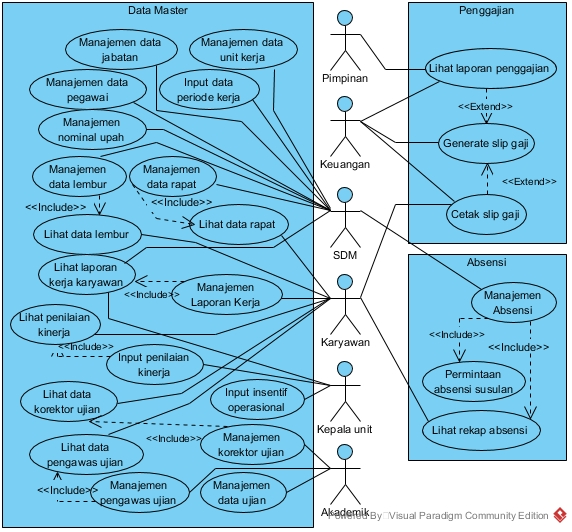
\includegraphics[width=15cm]{gambar/use-case-diagram}
    		            \caption{\emph{Use Case Diagram}}
    		            \label{usecase}
    		            \end{figure}
    			    \end{enumerate}
			        
			
			\subsubsection{\emph{Activity Diagram}}
			Berikut adalah perancangan \emph{activity diagram} yang peneliti lakukan dalam menggambarkan aktivitas masing-masing aktor dalam Sistem Informasi Penggajian Universitas Proklamasi 45:
			\begin{enumerate}
			    \itemsep0em
			    \item \emph{Activity Diagram Login}
			        \begin{figure}[H]
            		    \centering            		    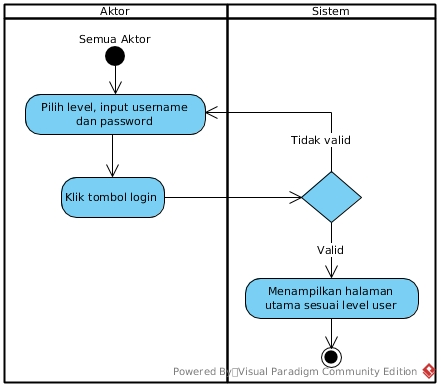
\includegraphics[width=13cm]{gambar/activity/login-activity}
            		    \caption{\emph{Activity Diagram Login}}
            		    \label{activity_login}
            		\end{figure}
            		\emph{Activity Diagram} pada Gambar \ref{activity_login} menjelaskan bagaimana aktor masuk ke dalam sistem. Pada halaman \emph{Login}, aktor akan memilih level \emph{user}, memasukan \emph{Username} dan \emph{Password}. Kemudian sistem akan melakukan validasi data. Apabila data valid, sistem akan menampilkan halaman Dashboard. Sedangkan apabila data yang dimasukan tidak valid, sistem akan kembali ke halaman \emph{Login} dan menampilkan pesan kesalahan.\newpage
			    \item \emph{Activity Diagram} Manajemen Data Karyawan
			        \begin{figure}[H]
            		    \centering            		    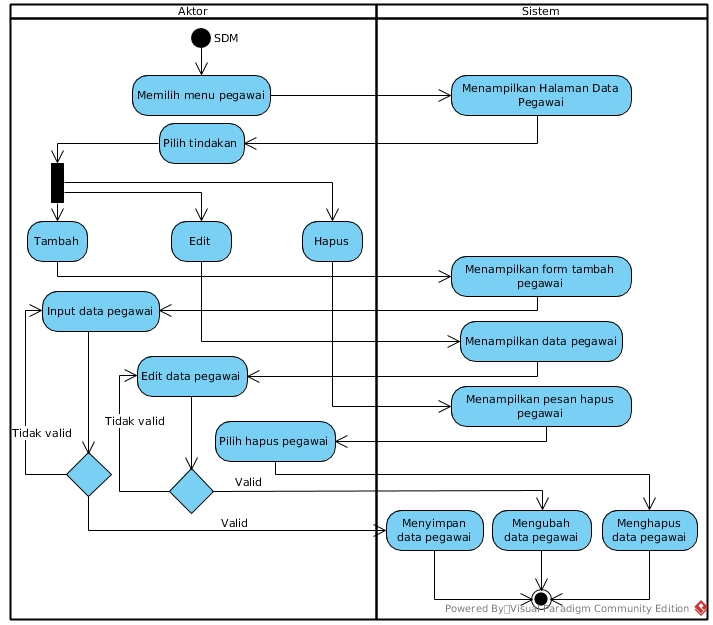
\includegraphics[width=14cm]{gambar/activity/manajemen-data-pegawai}
            		    \caption{\emph{Activity Diagram} Manajemen Data Karyawan}
            		    \label{activity_manajemen_pegawai}
            		\end{figure}
            		\emph{Activity Diagram} pada Gambar \ref{activity_manajemen_pegawai} menjelaskan bagaimana SDM melakukan manajemen data karyawan. Langkah pertama adalah memilih menu data karyawan dan sistem akan menampilkan halaman data karyawan. Manajemen data karyawan yang dimaksud adalah proses menambah, mengubah serta menghapus data karyawan. Ketika memilih tindakan tambah data karyawan, sistem akan menampilkan \emph{form} penambahan data yang berisi \emph{input field} yang harus diisi oleh SDM. Dalam melakukan tindakan tambah dan edit data karyawan, data akan divalidasi oleh sistem sebelum data disimpah atau diubah ke dalam \emph{database}.\newpage
            	\item \emph{Activity Diagram} Manajemen Data Unit Kerja
			        \begin{figure}[H]
            		    \centering            		     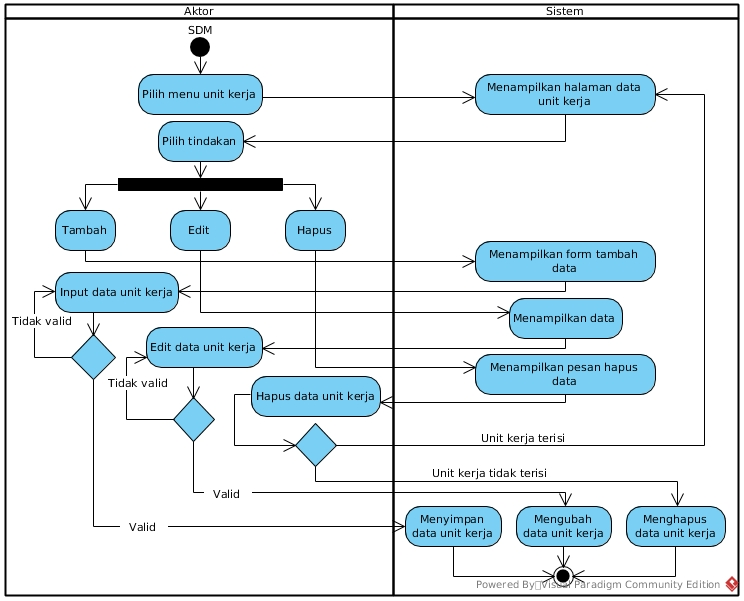
\includegraphics[width=14cm]{gambar/activity/manajemen-unit-kerja}
            		    \caption{\emph{Activity Diagram} Manajemen Unit Kerja}
            		    \label{activity_manajemen_unit}
            		\end{figure}
            		Dalam sebuah perusahaan pastinya perlu adanya bidang-bidang atau unit kerja yang mempunyai ranah kerja masing-masing. \emph{Activity Diagram} pada Gambar \ref{activity_manajemen_unit} menjelaskan bagaimana SDM melakukan manajemen data unit kerja karyawan, Pada setiap proses menambah data, mengubah data dan menghapus data unit kerja, sistem akan melakukan validasi data terlebih dahulu sebelum memproses tindakan tersebut. Seperti ketika ingin menghapus data unit kerja, apabila unit kerja terisi oleh karyawan, maka sistem akan membatalkan proses penghapusan tersebut. \newpage
            	\item \emph{Activity Diagram} Manajemen Data Jabatan
			        \begin{figure}[H]
            		    \centering
            		    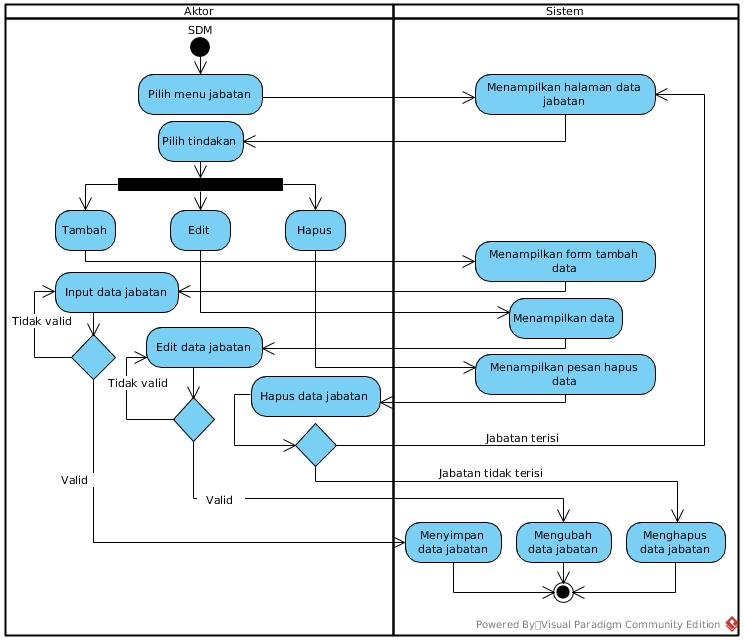
\includegraphics[width=14cm]{gambar/activity/manajemen-data-jabatan}
            		    \caption{\emph{Activity Diagram} Manajemen Data Jabatan}
            		    \label{activity_manajemen_jabatan}
            		\end{figure}
            		\emph{Activity Diagram} pada Gambar \ref{activity_manajemen_jabatan} menjelaskan bagaimana SDM melakukan manajemen data jabatan. Pada setiap proses menambah data, mengubah data dan menghapus data jabatan, sistem akan melakukan validasi data terlebih dahulu sebelum memproses tindakan tersebut. Seperti ketika ingin menghapus data jabatan, apabila jabatan tersebut terisi oleh karyawan, maka sistem akan membatalkan proses penghapusan tersebut. \newpage
            	\item \emph{Activity Diagram} Managemen Status Kepegawaian Pegawai
            	    \begin{figure}[H]
            		    \centering
            		    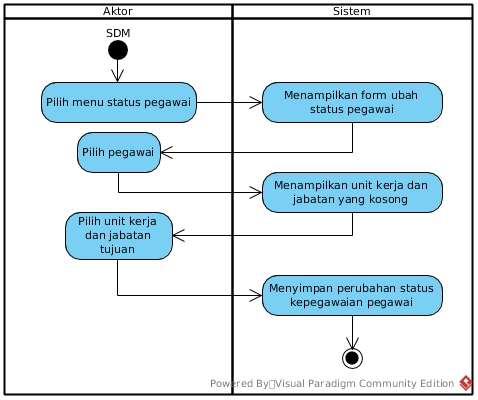
\includegraphics[width=14cm]{gambar/activity/manajemen-status-pegawai}
            		    \caption{\emph{Activity Diagram} Manajemen Status Kepegawaian Pegawai}
            		    \label{activity_status_pegawai}
            		\end{figure}
            		\emph{Activity Diagram} pada Gambar \ref{activity_status_pegawai} menjelaskan bagaimana proses SDM melakukan perubahan status kepegawaian pegawai, dalam hal ini unit kerja dan jabatan pegawai. SDM memilih menu status pegawai dan sistem akan menampilkan form ubah status pegawai. Kemudian SDM memilih pegawai yang akan diubah status kepegawaiannya dan sistem akan menampilkan data unit kerja dan jabatan yang kosong. SDM memilih unit kerja dan jabatan tujuan kemudian sistem akan menyimpan perubahan status kepegawaian pegawai tersebut. \newpage
            	\item \emph{Activity Diagram} Input Data Periode Kerja
            	    \begin{figure}[H]
            		    \centering
            		    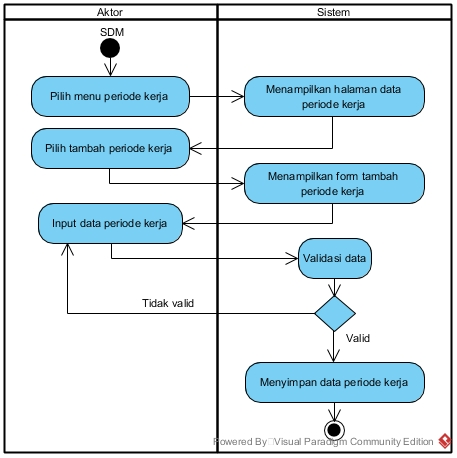
\includegraphics[width=13cm]{gambar/activity/input-data-periode-kerja}
            		    \caption{\emph{Activity Diagram} Input Data Periode Kerja}
            		    \label{activity_periode_kerja}
            		\end{figure}
            		\emph{Activity Diagram} pada Gambar \ref{activity_periode_kerja} menjelaskan bagaimana SDM melakukan \emph{input} data periode kerja. Pertama SDM akan memilih menu periode kerja dan sistem akan menampilkan halaman data periode kerja. Kemudian SDM memilih tindakan tambah periode kerja dan sistem akan menampilkan \emph{form} tambah periode kerja. Pada \emph{form} tersebut SDM mengisikan data-data periode kerja. Sebelum data periode kerja disimpan, sistem akan melakukan validasi data tersebut terlebih dahulu. \newpage
            	\item \emph{Activity Diagram} Manajemen Data Rapat
            	
            	Dalam proses manajemen data rapat terdapat beberapa \emph{activity} yang meliputi input data rapat, rekap upah rapat, dan lihat data rapat. Detail dari masing-masing \emph{activity} tersebut adalah sebagai berikut:
            	\begin{enumerate}[label=\alph*.]
            	    \itemsep0em
            	    \item Input Data Rapat
            	    \begin{figure}[H]
            		    \centering            		    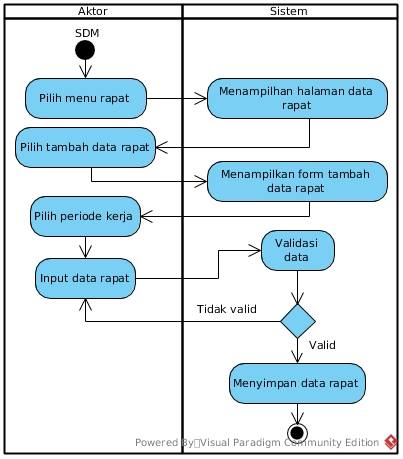
\includegraphics[width=11cm]{gambar/activity/input-data-rapat}
            		    \caption{\emph{Activity Diagram} Input Data Rapat}
            		    \label{activity_input_rapat}
            		\end{figure}
            		\emph{Activity Diagram} pada Gambar \ref{activity_input_rapat} menjelaskan bagaimana SDM melakukan penambahan data rapat karyawan. SDM memilih menu rapat dan sistem akan menampilkan halaman data rapat. Ketika memilih tambah data rapat, sistem akan menampilkan \emph{form} tambah data rapat. Kemudian SDM mengisi data rapat dan sistem akan melakukan validasi sebelum data disimpan.
            		\item Rekap Upah Rapat
            		\begin{figure}[H]
            		    \centering            		    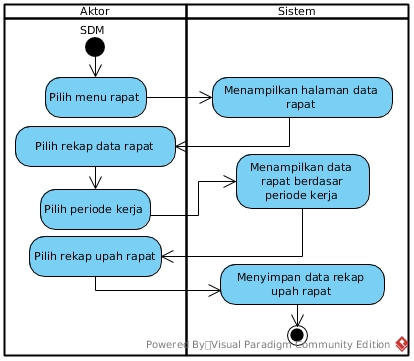
\includegraphics[width=11cm]{gambar/activity/rekap-upah-rapat}
            		    \caption{\emph{Activity Diagram} Rekap Upah Rapat}
            		    \label{activity_rekap_rapat}
            		\end{figure}
            		\emph{Activity Diagram} pada Gambar \ref{activity_rekap_rapat} menjelaskan bagaimana proses SDM melakukan perekapan upah rapat karyawan. Pada halaman data rapat SDM memilih rekap data rapat, lalu memilih periode kerja. Sistem akan menampilkan data rapat berdasarkan periode kerja yang dipilih. Setelah itu SDM dapat melakukan perekapan upah rapat selama satu periode yang dipilih.\newpage
            		\item Lihat Data Rapat
            		\begin{figure}[H]
            		    \centering            		    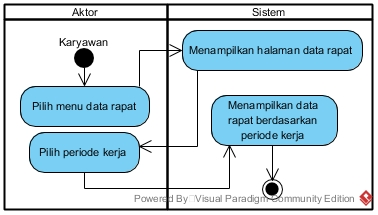
\includegraphics[width=11cm]{gambar/activity/lihat-data-rapat}
            		    \caption{\emph{Activity Diagram} Lihat Data Rapat}
            		    \label{activity_lihat_rapat}
            		\end{figure}
            		\emph{Activity Diagram} pada Gambar \ref{activity_lihat_rapat} menjelaskan bagaimana proses karyawan melihat data rapat yang dihadirinya. Pertama karyawan memilih menu data rapat dan sistem akan menampilkan halaman data rapat. Karyawan kemudian memilih periode kerja terlebih dahulu. Setelah itu sistem akan menampilkan data rapat karyawan sesuai dengan periode kerja yang dipilih.
            	\end{enumerate}
            	
            	\item \emph{Activity Diagram} Manajemen Data Lembur
            	
            	Dalam proses manajemen data lembur karyawan terdapat beberapa \emph{activity} yang meliputi input data lembur, rekap upah lembur, dan lihat data lembur. Detail dari masing-masing \emph{activity} tersebut adalah sebagai berikut: \newpage
            	\begin{enumerate}[label=\alph*.]
            	    \itemsep0em
            	    \item Input Data Lembur
            	    \begin{figure}[H]
            		    \centering            		    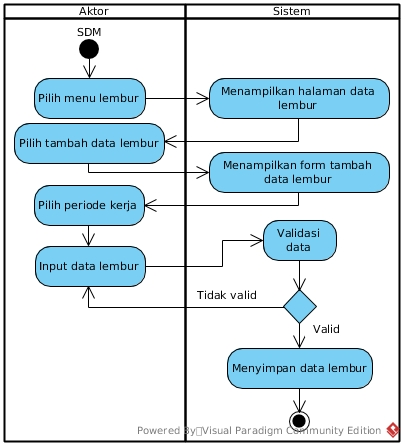
\includegraphics[width=11cm]{gambar/activity/input-data-lembur}
            		    \caption{\emph{Activity Diagram} Input Data Lembur}
            		    \label{activity_input_lembur}
            		\end{figure}
            		\emph{Activity Diagram} pada Gambar \ref{activity_input_lembur} menjelaskan bagaimana proses SDM melakukan penambahan data lembur karyawan. SDM memilih menu lembur dan sistem akan menampilkan halaman data lembur. Ketika SDM memilih tambah data lembur, sistem akan menampilkan \emph{form} tambah data lembur. Kemudian SDM memilih periode kerja dan mengisi data lembur. Setelah itu sistem akan melakukan validasi sebelum data lembur tersebut disimpan.\newpage
            	    \item Rekap Upah Lembur
            	    \begin{figure}[H]
            		    \centering            		    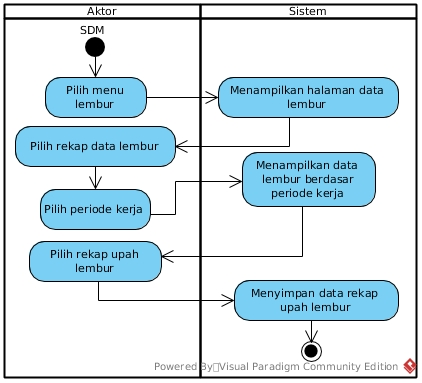
\includegraphics[width=11cm]{gambar/activity/rekap-upah-lembur}
            		    \caption{\emph{Activity Diagram} Rekap Upah Lembur}
            		    \label{activity_rekap_lembur}
            		\end{figure}
            		\emph{Activity Diagram} pada Gambar \ref{activity_rekap_lembur} menjelaskan bagaimana proses SDM melakukan perekapan upah lembur karyawan. Pada halaman data lembur SDM memilih rekap data lembur. Kemudian SDM memilih periode kerja dan sistem akan menampilkan data lembur karyawan berdasarkan periode kerja yang dipilih. Setelah itu SDM dapat melakukan perekapan upah lembur karyawan selama satu periode yang dipilih.\newpage
            	    \item Lihat Data Lembur
            	    \begin{figure}[H]
            		    \centering            		    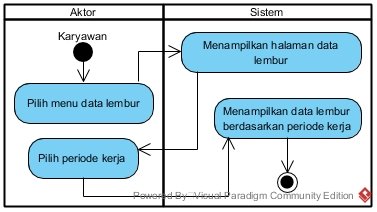
\includegraphics[width=11cm]{gambar/activity/lihat-data-lembur}
            		    \caption{\emph{Activity Diagram} Lihat Data Lembur}
            		    \label{activity_lihat_lembur}
            		\end{figure}
            		\emph{Activity Diagram} pada Gambar \ref{activity_lihat_lembur} menjelaskan bagaimana proses karyawan melihat data lembur yang dilakukannya. Pertama karyawan memilih menu data lembur dan sistem akan menampilkan halaman data lembur. Karyawan kemudian memilih periode kerja terlebih dahulu. Setelah itu sistem akan menampilkan data lembur karyawan sesuai dengan periode kerja yang dipilih.
            	\end{enumerate}
            	    
            	\item \emph{Activity Diagram} Manajemen Data Absensi
            	
            	Dalam proses manajemen data absensi karyawan terdiri dari beberapa \emph{activity} yang meliputi \emph{upload} data absensi dan ubah data absensi yang dapat dilakukan oleh SDM, serta lihat data absensi yang dapat dilakukan oleh karyawan. Detail dari masing-masing \emph{activity} tersebut adalah sebagai berikut: \newpage
            	\begin{enumerate}[label=\alph*.]
            	    \itemsep0em
            	    \item \emph{Upload} Data Absensi
            	    \begin{figure}[H]
            		    \centering            		    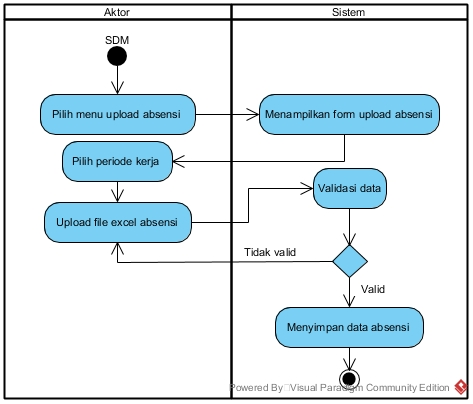
\includegraphics[width=13cm]{gambar/activity/upload-absensi}
            		    \caption{\emph{Activity Diagram} Upload Absensi}
            		    \label{activity_upload_absensi}
            		\end{figure}
            		\emph{Activity Diagram} pada Gambar \ref{activity_upload_absensi} menjelaskan bagaimana SDM melakukan proses \emph{upload} atau pengunggahan data absensi karyawan. SDM memilih tindakan \emph{upload} absensi dan sistem akan menampilkan \emph{form upload} absensi. Sebelum memilih file, SDM terlebih dahulu memilih periode kerja sesuai dengan periode kerja yang sedang berjalan. Sistem akan melakukan validasi terlebih dahulu sebelum data absensi tersebut disimpan.\newpage
            	    \item Ubah Data Absensi
            	    \begin{figure}[H]
            		    \centering            		    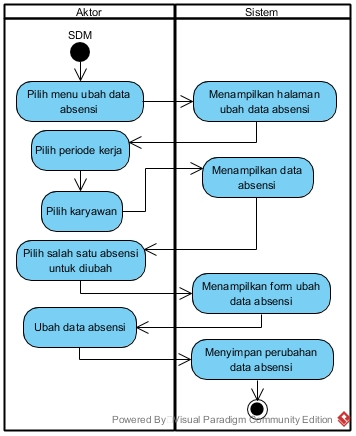
\includegraphics[width=11cm]{gambar/activity/ubah-data-absensi}
            		    \caption{\emph{Activity Diagram} Ubah Data Absensi}
            		    \label{activity_ubah_absensi}
            		\end{figure}
            		\emph{Activity Diagram} pada Gambar \ref{activity_ubah_absensi} menjelaskan bagaimana proses SDM melakukan perubahan data absensi karyawan. SDM memilih menu ubah data absensi dan sistem akan menampilkan halaman ubah data absensi. Kemudian SDM memilih karyawan dan periode kerja. Setelah itu sistem akan menampilkan data absensi sesuai karyawan dan periode yang dipilih. SDM memilih salah satu data absensi yang akan dilakukan perubahan. Sistem akan menampilkan \emph{form} ubah data absensi. Setelah itu SDM dapat mengubah data absensi yang dipilih dan sistem akan menyimpan perubahan data absensi tersebut.
            	    \item Lihat Rekap Absensi
            	    \begin{figure}[H]
            		    \centering            		    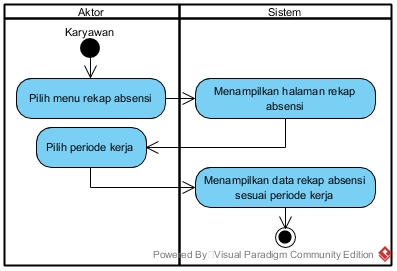
\includegraphics[width=11cm]{gambar/activity/lihat-data-rekap-absensi}
            		    \caption{\emph{Activity Diagram} Lihat Data Rekap Absensi}
            		    \label{activity_lihat_absensi}
            		\end{figure}
            		\emph{Activity Diagram} pada Gambar \ref{activity_lihat_absensi} menjelaskan bagaimana proses karyawan melihat data rekap absensi. Karyawan memilih menu data rekap absensi dan sistem akan menampilkan halaman rekap absensi. Kemudian karyawan memilih periode kerja terlebih dahulu. Setelah itu sistem akan menampilkan data rekap absensi karyawan tersebut sesuai periode kerja yang dipilih.
            	\end{enumerate}
            	    
            	\item \emph{Activity Diagram} Manajemen Data Ujian
            	
            	Dalam proses manajemen data ujian terdapat beberapa \emph{activity} yang meliputi input data ujian, input pengawas ujian, input korektor ujian, rekap upah pengawas ujian, rekap upah korektor ujian, lihat data pengawas ujian dan lihat data korektor ujian. Detail dari masing-masing \emph{activity} tersebut adalah sebagai berikut: \newpage
            	\begin{enumerate}[label=\alph*.]
            	    \itemsep0em
            	    \item Input Data Ujian
            	    \begin{figure}[H]
            		    \centering            		    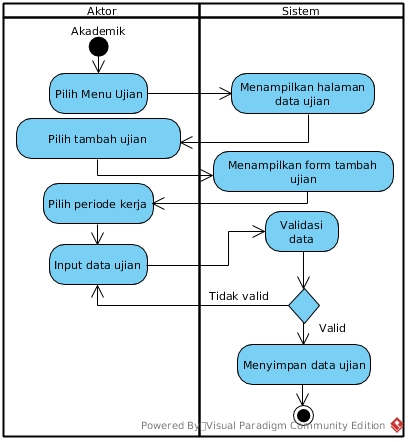
\includegraphics[width=11cm]{gambar/activity/input-data-ujian}
            		    \caption{\emph{Activity Diagram} Input Data Ujian}
            		    \label{activity_input_ujian}
            		\end{figure}
            		\emph{Activity Diagram} pada Gambar \ref{activity_input_ujian} menjelaskan bagaimana staf Akademik melakukan \emph{input} data ujian. Staf Akademik memilih menu ujian dan sistem menampilkan halaman data ujian. Ketika memilih tambah ujian, sistem akan menampilkan form tambah data ujian. Staf akademik memilih periode kerja dan mengisi data ujian, kemudian sistem akan melakukan validasi sebelum data disimpan ke dalam \emph{database}.\newpage
            		\item Input Data Pengawas Ujian
            		\begin{figure}[H]
            		    \centering            		    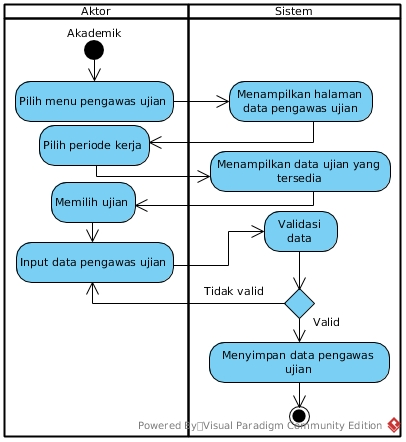
\includegraphics[width=11cm]{gambar/activity/input-data-pengawas-ujian}
            		    \caption{\emph{Activity Diagram} Input Data Pengawas Ujian}
            		    \label{activity_input_pengawas}
            		\end{figure}
            		\emph{Activity Diagram} pada Gambar \ref{activity_input_pengawas} menjelaskan bagaimana staf Akademik melakukan proses input data pengawas ujian. Sebelum staf Akademik melakukan input data, staf Akademik perlu memilih periode kerja terlebih dahulu. Kemudian sistem akan menampilkan data ujian yang tersedia sesuai dengan periode kerja dan staff Akademik memilih ujian yang akan di input data pengawasnya. Sistem akan melakukan validasi sebelum menyimpan data pengawas ujian tersebut.\newpage
            		\item Input Data Korektor Ujian
            		\begin{figure}[H]
            		    \centering            		    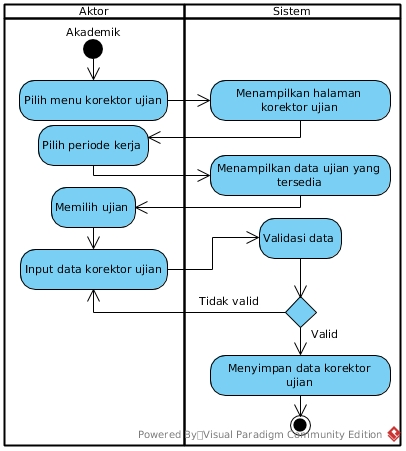
\includegraphics[width=11cm]{gambar/activity/input-data-korektor-ujian}
            		    \caption{\emph{Activity Diagram} Input Data Korektor Ujian}
            		    \label{activity_input_korektor}
            		\end{figure}
            		\emph{Activity Diagram} pada Gambar \ref{activity_input_korektor} menjelaskan bagaimana staf Akademik melakukan proses input data korektor ujian. Sebelum staf Akademik melakukan input data korektor ujian, staf Akademik perlu memilih periode kerja terlebih dahulu. Sistem akan menampilkan data ujian yang tersedia sesuai dengan periode kerja dan staff Akademik memilih ujian yang akan di input data korektornya. Kemudian sistem akan melakukan validasi sebelum menyimpan data korektor ujian tersebut.\newpage
            		\item Rekap Upah Pengawas Ujian
            		\begin{figure}[H]
            		    \centering            		    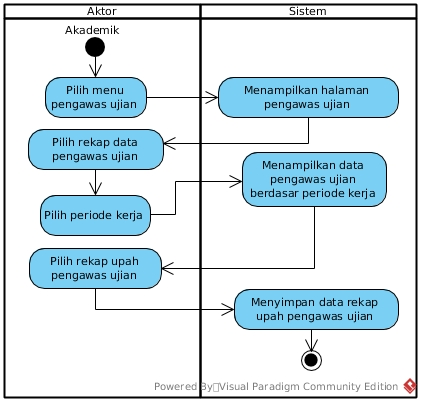
\includegraphics[width=11cm]{gambar/activity/rekap-upah-pengawas}
            		    \caption{\emph{Activity Diagram} Rekap Upah Pengawas Ujian}
            		    \label{activity_rekap_pengawas}
            		\end{figure}
            		\emph{Activity Diagram} pada Gambar \ref{activity_rekap_pengawas} menjelaskan bagaimana proses staf Akademik melakukan perekapan upah pengawas ujian. Pertama, pada halaman pengawas ujian staf Akademik memilih rekap data pengawas ujian. Kemudian staf Akademik memilih periode kerja dan sistem akan menampilkan data pengawas ujian berdasarkan periode kerja yang dipilih. Setelah itu staf Akademik dapat melakukan perekapan upah pengawas ujian selama satu periode yang dipilih.\newpage
            		\item Rekap Upah Korektor Ujian
            		\begin{figure}[H]
            		    \centering            		    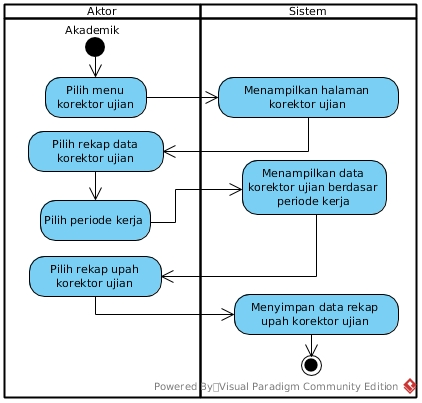
\includegraphics[width=11cm]{gambar/activity/rekap-upah-korektor}
            		    \caption{\emph{Activity Diagram} Rekap Upah Korektor Ujian}
            		    \label{activity_rekap_korektor}
            		\end{figure}
            		\emph{Activity Diagram} pada Gambar \ref{activity_rekap_korektor} menjelaskan bagaimana proses staf Akademik melakukan perekapan upah korektor ujian. Pada halaman korektor ujian staf Akademik memilih rekap data korektor ujian. Kemudian staf Akademik memilih periode kerja dan sistem akan menampilkan data korektor ujian berdasarkan periode kerja yang dipilih. Setelah itu staf Akademik dapat melakukan perekapan upah korektor ujian selama satu periode yang dipilih.\newpage
            		\item Lihat Data Pengawas Ujian
            	    \begin{figure}[H]
            		    \centering            		    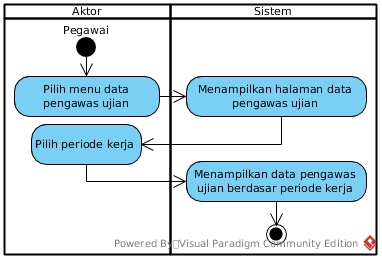
\includegraphics[width=11cm]{gambar/activity/lihat-data-pengawas-ujian}
            		    \caption{\emph{Activity Diagram} Lihat Data Pengawas Ujian}
            		    \label{activity_lihat_pengawas}
            		\end{figure}
            		\emph{Activity Diagram} pada Gambar \ref{activity_lihat_pengawas} menjelaskan bagaimana proses karyawan melihat data pengawas ujian. Karyawan memilih menu data pengawas ujian dan sistem menampilkan halaman pengawas ujian. Kemudian karyawan memilih periode kerja terlebih dahulu dan sistem akan menampilkan data pengawas ujian dari karyawan tersebut sesuai periode kerja yang dipilih.\newpage
            		\item Lihat Data Korektor Ujian
            	    \begin{figure}[H]
            		    \centering            		    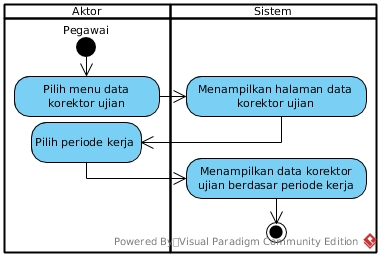
\includegraphics[width=11cm]{gambar/activity/lihat-data-korektor-ujian}
            		    \caption{\emph{Activity Diagram} Lihat Data Korektor Ujian}
            		    \label{activity_lihat_korektor}
            		\end{figure}
            		\emph{Activity Diagram} pada Gambar \ref{activity_lihat_korektor} menjelaskan bagaimana proses karyawan melihat data korektor ujian. Karyawan memilih menu data korektor ujian dan sistem menampilkan halaman korektor ujian. Kemudian karyawan memilih periode kerja terlebih dahulu dan sistem akan menampilkan data korektor ujian dari karyawan tersebut sesuai periode kerja yang dipilih.
            	\end{enumerate}
            	
            	\item \emph{Activity Diagram} Manajemen Laporan Kerja
            	
            	Dalam proses manajemen data laporan kerja karyawan terdapat beberapa \emph{activity} yang terdiri dari kategori input data dan kategori lihat data. Kategori input data meliputi input rencana kerja harian, input laporan kerja harian, input checklist bulanan dan input laporan kerja bulanan. Untuk kategori lihat data meliputi melihat seluruh laporan kerja baik harian maupun bulanan dan melihat detail kegiatan dari laporan kerja tersebut. Detail dari masing-masing \emph{activity} tersebut adalah sebagai berikut:\newpage
            		\begin{enumerate}[label=\alph*.]
            		    \itemsep0em
            		    \item Input Rencana Kerja Harian
            		    \begin{figure}[H]
                		    \centering                		    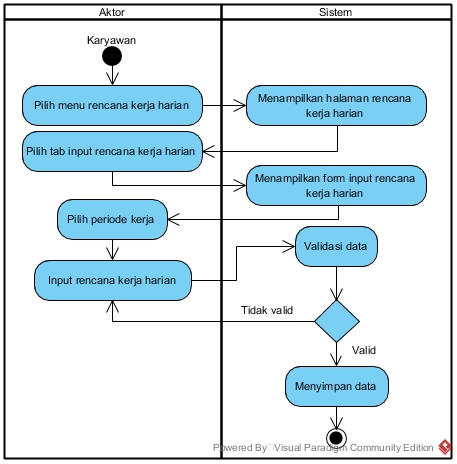
\includegraphics[width=11cm]{gambar/activity/input-rencana-kerja-harian}
                		    \caption{\emph{Activity Diagram} Input Rencana Kerja Harian}
                		    \label{activity_input_rkh}
                		\end{figure}
                		\emph{Activity Diagram} pada Gambar \ref{activity_input_rkh} menjelaskan bagaimana proses karyawan melakukan input data rencana kerja harian (RKH). Karyawan memilih menu RKH dan sistem akan menampilkan halaman data RKH. Kemudian karyawan memilih input RKH dan sistem akan menampilkan \emph{form} input RKH. Karyawan memilih periode kerja dan mengisi data RKH. Sistem akan melakukan validasi sebelum data RKH disimpan ke dalam \emph{database}.\newpage
            		    \item Input Laporan Kerja Harian
            		    \begin{figure}[H]
                		    \centering                		    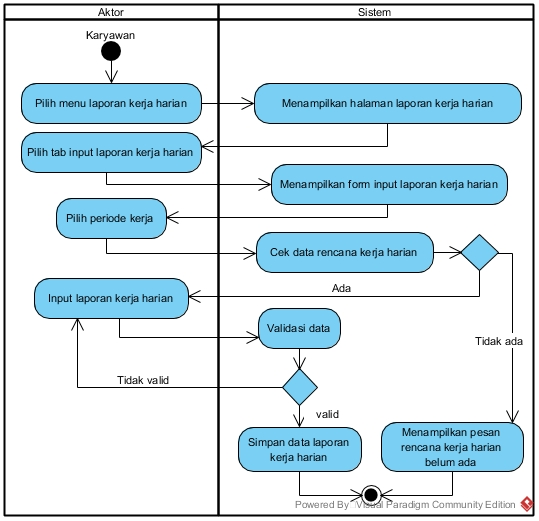
\includegraphics[width=11cm]{gambar/activity/input-laporan-kerja-harian}
                		    \caption{\emph{Activity Diagram} Input Laporan Kerja Harian}
                		    \label{activity_input_lh}
                		\end{figure}
                		\emph{Activity Diagram} pada Gambar \ref{activity_input_lh} menjelaskan bagaimana proses karyawan melakukan input data laporan kerja harian (LH). Karyawan memilih menu LH dan sistem akan menampilkan halaman data LH. Kemudian karyawan memilih input LH dan sistem akan menampilkan \emph{form} input LH. Karyawan memilih periode kerja dan sistem akan melakukan pengecekan data RKH sudah ada atau belum. Apabila RKH sudah ada, sistem akan menampilkan data RKH yang siap diisi LH-nya. Sistem akan melakukan validasi sebelum data LH disimpan ke dalam \emph{database}.\newpage
            		    \item Input Checklist Bulanan
            		    \begin{figure}[H]
                		    \centering                		    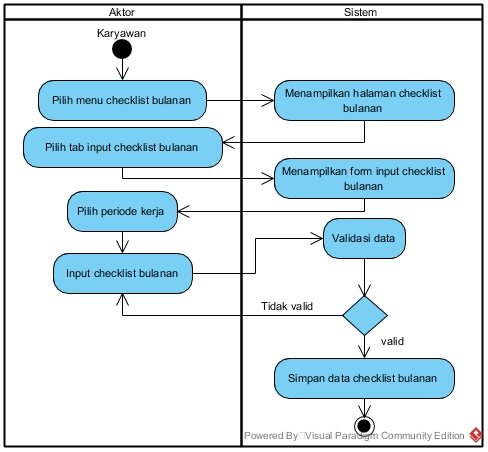
\includegraphics[width=11cm]{gambar/activity/input-checklist-bulanan}
                		    \caption{\emph{Activity Diagram} Input Checklist Bulanan}
                		    \label{activity_input_checklist}
                		\end{figure}
                		\emph{Activity Diagram} pada Gambar \ref{activity_input_checklist} menjelaskan bagaimana proses karyawan melakukan input data checklist bulanan (CB). Karyawan memilih menu CB dan sistem akan menampilkan halaman data CB. Kemudian karyawan memilih input CB dan sistem akan menampilkan \emph{form} input CB. Karyawan memilih periode kerja dan mengisi data CB. Sistem akan melakukan validasi sebelum data CB disimpan ke dalam \emph{database}.\newpage
            		    \item Input Laporan Kerja Bulanan
            		    \begin{figure}[H]
                		    \centering                		    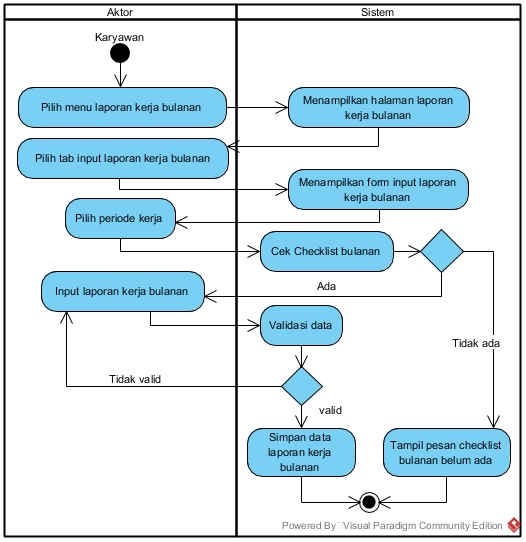
\includegraphics[width=11cm]{gambar/activity/input-laporan-kerja-bulanan}
                		    \caption{\emph{Activity Diagram} Input Laporan Kerja Bulanan}
                		    \label{activity_input_lb}
                		\end{figure}
                		\emph{Activity Diagram} pada Gambar \ref{activity_input_lb} menjelaskan bagaimana proses karyawan melakukan input data laporan kerja bulanan (LB). Karyawan memilih menu LB dan sistem akan menampilkan halaman data LB. Kemudian karyawan memilih input LB dan sistem akan menampilkan \emph{form} input LB. Karyawan memilih periode kerja dan sistem akan melakukan pengecekan data CB sudah ada atau belum. Apabila data CB sudah ada, sistem akan menampilkan data CB yang siap diisi LB-nya. Sistem akan melakukan validasi sebelum data LB disimpan ke dalam \emph{database}.\newpage
                		\item Lihat Laporan Kerja Karyawan
                		\begin{figure}[H]
            		        \centering            		    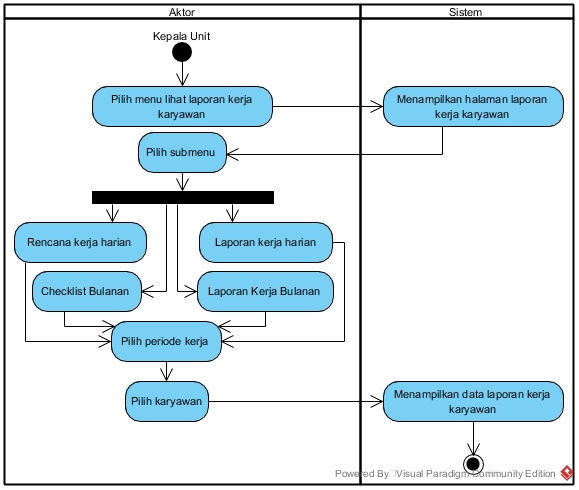
\includegraphics[width=13cm]{gambar/activity/lihat-laporan-kerja-pegawai}
            		        \caption{\emph{Activity Diagram} Lihat Laporan Kerja Karyawan}
            		        \label{activity_lihat_laporan_kerja}
            		    \end{figure}
            		    \emph{Activity Diagram} pada Gambar \ref{activity_lihat_laporan_kerja} menjelaskan bagaimana proses Kepala Unit melihat laporan kerja karyawan yang dibawahinya. Kepala Unit memilih menu laporan kerja karyawan dan sistem menampilkan halaman laporan kerja karyawan. Kemudian memilih antara laporan kerja harian atau laporan kerja bulanan. Setelah itu Kepala Unit memilih periode kerja dan nama karyawan yang dibawahinya. Sistem akan menampilkan data laporan kerja karyawan sesuai periode dan nama karyawan yang dipilih.\newpage
            		\end{enumerate}
            	
            	\item \emph{Activity Diagram} Manajemen Penilaian Kinerja Karyawan
            	
            	Dalam proses manajemen penilaian kinerja karyawan terdapat beberapa \emph{activity} yang meliputi input penilaian kinerja karyawan dan lihat data penilaian kinerja karyawan. Detail dari masing-masing \emph{activity} tersebut adalah sebagai berikut:
            	\begin{enumerate}[label=\alph*.]
            	    \itemsep0em
            	    \item Input Penilaian Kinerja Karyawan
            	    \begin{figure}[H]
            		    \centering
            		    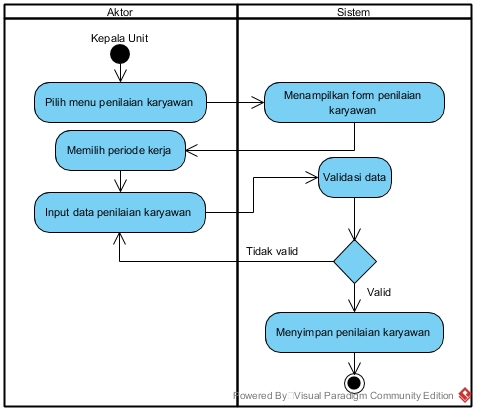
\includegraphics[width=11cm]{gambar/activity/input-penilaian-pegawai}
            		    \caption{\emph{Activity Diagram} Input Penilaian Kinerja Karyawan}
            		    \label{activity_input_penilaian}
            		\end{figure}
            		\emph{Activity Diagram} pada Gambar \ref{activity_input_penilaian} menjelaskan bagaimana Kepala Unit memberikan penilaian kinerja kepada karyawan yang dibawahinya. Kepala Unit memilih menu penilaian kinerja dan sistem akan menampilkan form penilaian karyawan. Sebelum input data penilaian, Kepala Unit harus memilih periode kerja terlebih dahulu. Sistem akan melakukan validasi sebelum data penilaian kinerja disimpan ke dalam sistem.
            	    \item Lihat Data Penilaian Kinerja Karyawan
            	    \begin{figure}[H]
            		    \centering
            		    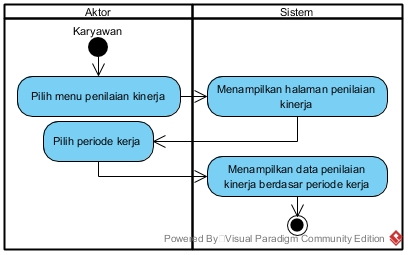
\includegraphics[width=9cm]{gambar/activity/lihat-data-penilaian-kinerja}
            		    \caption{\emph{Activity Diagram} Lihat Data Penilaian Kinerja}
            		    \label{activity_lihat_penilaian}
            		\end{figure}
            		\emph{Activity Diagram} pada Gambar \ref{activity_lihat_penilaian} menjelaskan proses bagaimana karyawan melihat data penilaian kinerja. Karyawan memilih memilih periode kerja dan sistem akan menampilkan data sesuai periode kerja yang dipilih.
            	\end{enumerate}
            	    
            	\item \emph{Activity Diagram} Input Insentif Operasional
            	    \begin{figure}[H]
            		    \centering
            		    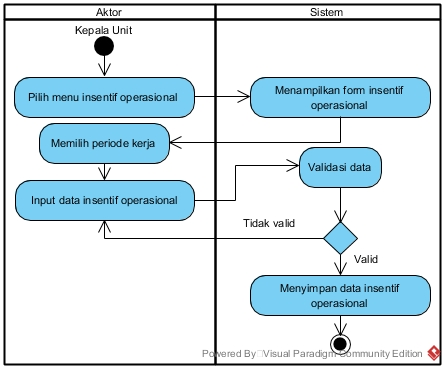
\includegraphics[width=10cm]{gambar/activity/input-insentif-operasional}
            		    \caption{\emph{Activity Diagram} Input Insentif Operasional}
            		    \label{activity_input_insentif}
            		\end{figure}
            		\emph{Activity Diagram} pada Gambar \ref{activity_input_insentif} menjelaskan bagaimana Kepala Unit memberikan insentif operasional kepada karyawan yang dibawahinya. Kepala Unit memilih menu insentif operasional dan sistem akan menampilkan form input insentif operasional. Sebelum input data insentif operasional, Kepala Unit harus memilih periode kerja terlebih dahulu. Sistem akan melakukan validasi sebelum data insentif operasional tersebut disimpan ke dalam sistem. 
            	 \item \emph{Activity Diagram} Manajemen Gaji Karyawan
            	 
            	 Proses manajemen gaji karyawan ini terdiri dari beberapa \emph{activity} yang meliputi \emph{generate} slip gaji, lihat data slip gaji, cetak slip gaji, dan lihat laporan penggajian. Detail dari masing-masing \emph{activity} tersebut adalah sebagai berikut:
                \begin{enumerate}[label=\alph*.]
            	     \itemsep0em
            	     \item \emph{Generate} Slip Gaji
            	     \begin{figure}[H]
            		    \centering
            		    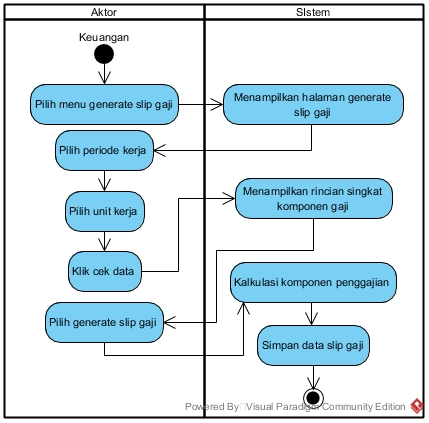
\includegraphics[width=10cm]{gambar/activity/generate-slip-gaji}
            		    \caption{\emph{Activity Diagram Generate} Slip Gaji}
            		    \label{activity_generate_slip}
                    \end{figure}
                    \emph{Activity Diagram} pada Gambar \ref{activity_generate_slip} menjelaskan bagaimana staf Keuangan melakukan \emph{generate} slip gaji karyawan. Di dalam halaman \emph{generate} slip gaji, staf Keuangan memilih periode kerja dan unit kerja, kemudian sistem akan menampilkan rincian komponen gaji karyawan. Setelah itu Keuangan dapat memilih \emph{generate} slip gaji, kemudian sistem akan menyimpan hasil kalkulasi dan data slip gaji tersebut.
            	    \item Cetak Slip Gaji
            	    \begin{figure}[H]
            		    \centering
            		    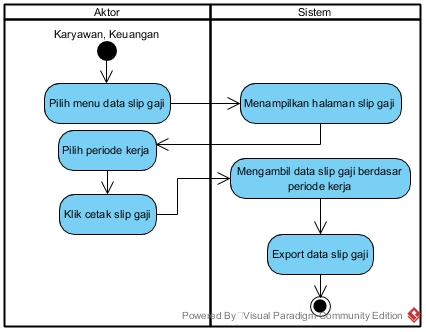
\includegraphics[width=10cm]{gambar/activity/cetak-slip-gaji}
            		    \caption{\emph{Activity Diagram} Cetak Slip Gaji}
            		    \label{activity_cetak_slip}
            		\end{figure}
            		\emph{Activity Diagram} pada Gambar \ref{activity_cetak_slip} menjelaskan bagaimana karyawan melakukan proses cetak slip gaji. Pada halaman cetak slip gaji, karyawan memilih periode kerja terlebih dahulu dan klik cetak slip gaji. Kemudian sistem akan mengambil data slip gaji berdasarkan periode yang dipilih dan melakukan \emph{export} data slip gaji tersebut.
            		\newpage
            		\item Lihat Laporan Penggajian
            		\begin{figure}[H]
            		    \centering
            		    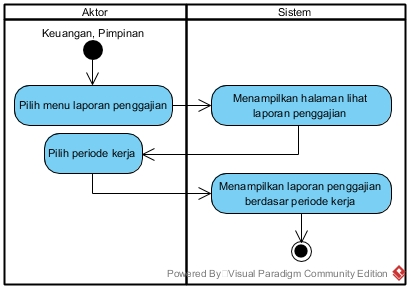
\includegraphics[width=10cm]{gambar/activity/lihat-laporan-penggajian}
            		    \caption{\emph{Activity Diagram} Lihat Laporan Penggajian}
            		    \label{activity_laporan_penggajian}
            		\end{figure}
            		\emph{Activity Diagram} pada Gambar \ref{activity_laporan_penggajian} menjelaskan bagaimana Keuangan dan Pimpinan melihat laporan penggajian karyawan. Pada halaman lihat laporan penggajian, kedua aktor tersebut memilih periode kerja terlebih dahulu. Setelah itu sistem akan mengambil dan menampilkan data laporan penggajian karyawan berdasarkan periode kerja yang dipilih.
                \end{enumerate}
			\end{enumerate}
			
			
			\subsubsection{\emph{Sequence Diagram}}
			Perancangan \emph{sequence} bertujuan untuk menjelaskan secara detail urutan proses yang dilakukan di dalam sistem untuk mencapai tujuan dari \emph{Use Case} yang telah digambarkan sebelumnya. Berikut \emph{Sequence Diagram} yang menggambarkan masing-masing \emph{sequence}:
			\newpage
			\begin{enumerate}
			    \itemsep0em
			    \item \emph{Sequence Diagram} Login
			        \begin{figure}[H]
            		    \centering
            		    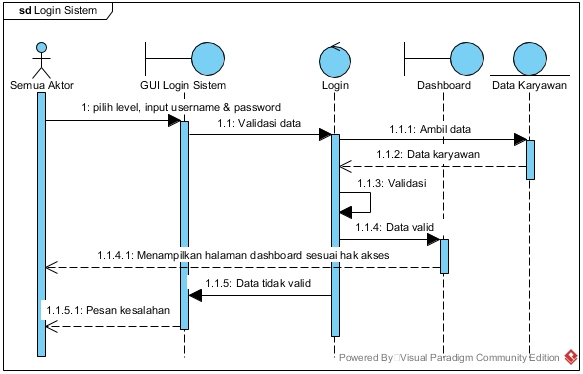
\includegraphics[width=13cm]{gambar/sequence/seq-login}
            		    \caption{\emph{Sequence Diagram} Login}
            		    \label{sequence_login}
            		\end{figure}
            		\emph{Sequence Diagram} pada Gambar \ref{sequence_login} menjelaskan bagaimana urutan proses semua Aktor \emph{Login} ke dalam sistem. Pertama Aktor harus memilih level atau hak aksesnya, kemudian memasukkan \emph{username} dan \emph{password}. Sistem akan melakukan validasi data tersebut berdasarkan data karyawan. Apabila level yang dipilih sesuai dengan \emph{username} dan \emph{password} maka sistem akan menampilkan halaman \emph{Dashboard} sesuai levelnya. Sedangkan apabila data yang dimasukan salah, sistem akan menampilkan pesan kesalahan. \newpage
			    \item \emph{Sequence Diagram} Manajemen Data Karyawan
			        \begin{figure}[H]
            		    \centering
            		    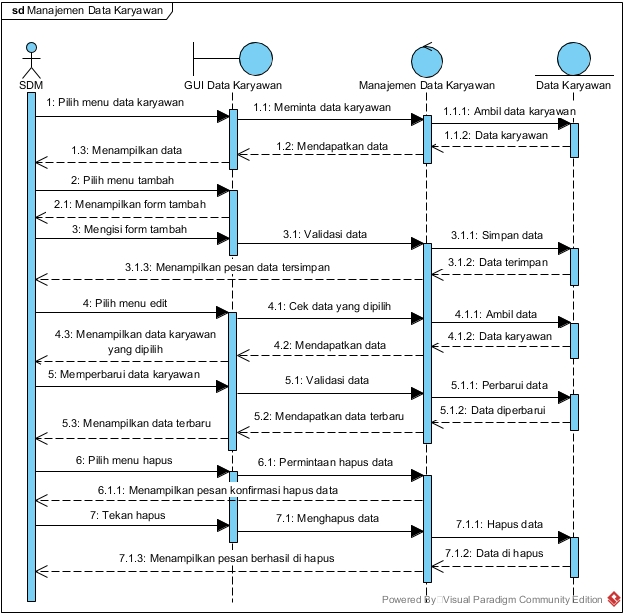
\includegraphics[width=14cm]{gambar/sequence/manajemen-pegawai}
            		    \caption{\emph{Sequence Diagram} Manajemen Data Karyawan}
            		    \label{sequence_manajemen_pegawai}
            		\end{figure}
            		\emph{Sequence Diagram} pada Gambar \ref{sequence_manajemen_pegawai} menjelaskan bagaimana urutan proses SDM melakukan manajemen data karyawan, meliputi tambah data, ubah data dan hapus data. Proses dimulai ketika SDM memilih menu data karyawan dan sistem akan meminta data karyawan untuk ditampilkan kepada SDM. Ketika memilih tambah karyawan, sistem akan menampilkan form yang akan diisi oleh SDM. Sebelum disimpan ke dalam \emph{database} karyawan, sistem akan melakukan validasi terlebih dahulu. Kemudian sistem akan menampilkan pesan apabila data berhasil disimpan ke dalam \emph{database}.
            		
            		Ketika memilih edit data karyawan, sistem akan menampilkan detail data karyawan yang dipilih dan SDM dapat mengubah data tersebut. Seperti tindakan tambah karyawan, sebelum mengubah data karyawan sistem juga akan melakukan validasi.
            		
            		Ketika SDM ingin menghapus data karyawan, sistem akan menampilkan pesan konfirmasi apakah data benar-benar ingin dihapus sebelum menekan tombol hapus.
            	\item \emph{Sequence Diagram} Manajemen Data Unit Kerja
			        \begin{figure}[H]
            		    \centering
            		    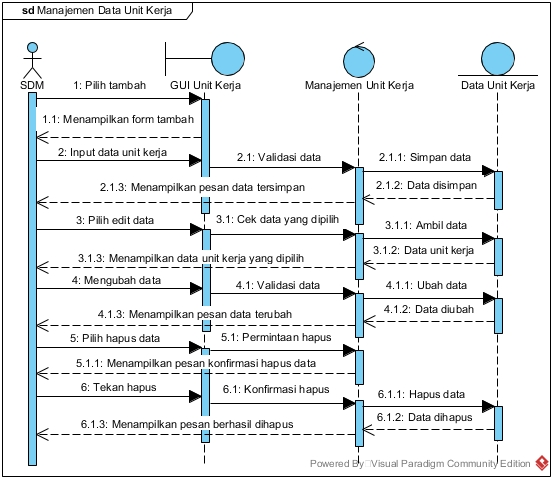
\includegraphics[width=13cm]{gambar/sequence/manajemen-unit-kerja}
            		    \caption{\emph{Sequence Diagram} Manajemen Data Unit Kerja}
            		    \label{sequence_manajemen_unitkerja}
            		\end{figure}
            		\emph{Sequence Diagram} pada Gambar \ref{sequence_manajemen_unitkerja} menjelaskan bagaimana urutan proses SDM melakukan manajemen data unit kerja, meliputi tambah data, ubah data dan hapus data. Ketika memilih tambah data, sistem akan menampilkan form dan SDM mengisi data unit kerja. Sistem akan melakukan validasi data sebelum disimpan dan akan menampilkan pesan apabila data berhasil disimpan ke dalam \emph{database} Unit Kerja.
            		
            		Pada pilihan edit data, sistem akan mengambil data unit kerja yang dipilih dan menampilkannya kepada SDM. Kemudian SDM dapat mengubah data tersebut dan menyimpannya. Sebelum disimpan sistem akan melakukan validasi terlebih dahulu. Sistem akan menampilkan pesan bahwa data berhasil diperbarui. Proses hapus data unit kerja sama dengan proses hapus data karyawan. Sistem akan menampilkan pesan konfirmasi terlebih dahulu.
            	\item \emph{Sequence Diagram} Manajemen Data Jabatan
			        \begin{figure}[H]
            		    \centering
            		    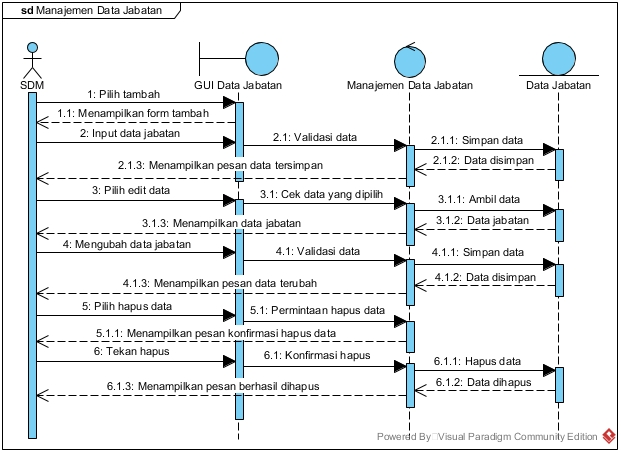
\includegraphics[width=13cm]{gambar/sequence/manajemen-jabatan}
            		    \caption{\emph{Sequence Diagram} Manajemen Data Jabatan}
            		    \label{sequence_manajemen_jabatan}
            		\end{figure}
            		\emph{Sequence Diagram} pada Gambar \ref{sequence_manajemen_jabatan} menjelaskan bagaimana urutan proses SDM melakukan manajemen data jabatan. Ketika memilih tambah data, sistem akan menampilkan form dan SDM mengisi data jabatan. Sistem akan melakukan validasi data sebelum disimpan dan akan menampilkan pesan apabila data berhasil disimpan ke dalam \emph{database} Jabatan.
            		
            		Pada pilihan edit data, sistem akan mengambil data jabatan yang dipilih dan menampilkannya kepada SDM. Kemudian SDM dapat mengubah data tersebut dan menyimpannya. Sebelum disimpan sistem akan melakukan validasi terlebih dahulu. Sistem akan menampilkan pesan bahwa data berhasil diperbarui. Proses hapus data jabatan sama dengan proses hapus data karyawan. Sistem akan menampilkan pesan konfirmasi terlebih dahulu.
            	\item \emph{Sequence Diagram} Manajemen Status Kepegawaian
			        \begin{figure}[H]
            		    \centering            		    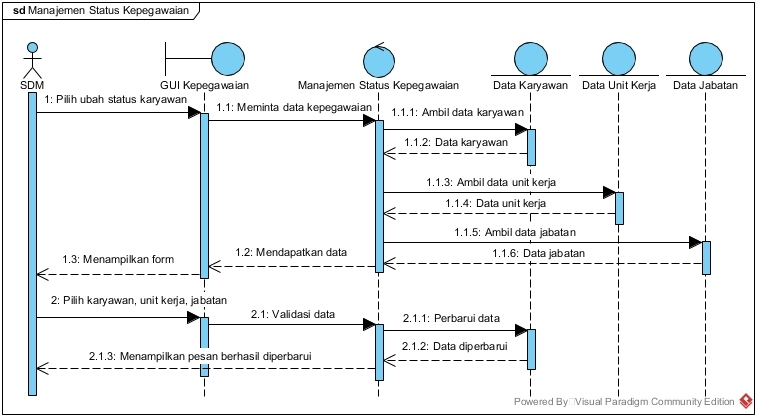
\includegraphics[width=14cm]{gambar/sequence/manajemen-status-kepegawaian}
            		    \caption{\emph{Sequence Diagram} Manajemen Status Kepegawaian}
            		    \label{sequence_manajemen_kepegawaian}
            		\end{figure}
            		\emph{Sequence Diagram} pada Gambar \ref{sequence_manajemen_kepegawaian} menjelaskan bagaimana urutan proses SDM melakukan manajemen status kepegawaian karyawan. Maksud dari status kepegawaian adalah unit kerja dan jabatan dari karyawan. Langkah pertama SDM memilih tindakan ubah status karyawan. Kemudian sistem akan mengambil data karyawan, data unit kerja dan data jabatan dari dalam \emph{database} untuk ditampilkan kepada SDM. Kemudian SDM memilih karyawan, data unit kerja dan data jabatan yang menjadi tujuan. Sistem akan melakukan validasi data sebelum data disimpan dan menampilkan pesan apabila data berhasil diperbarui ke dalam \emph{database}.
            	\item \emph{Sequence Diagram} Input Data Periode Kerja
			        \begin{figure}[H]
            		    \centering
            		    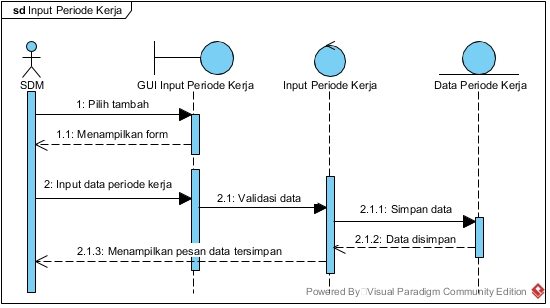
\includegraphics[width=13cm]{gambar/sequence/input-periode-kerja}
            		    \caption{\emph{Sequence Diagram} Input Data Periode Kerja}
            		    \label{sequence_input_periode}
            		\end{figure}
            		\emph{Sequence Diagram} pada Gambar \ref{sequence_input_periode} menjelaskan bagaimana urutan proses SDM melakukan \emph{input} data periode kerja. SDM memilih tambah data, dan sistem akan menampilkan \emph{form input} data. Kemudian SDM akan mengisi data periode kerja pada \emph{form} tersebut. Sistem akan melakukan validasi data terlebih dahulu sebelum disimpan ke dalam \emph{database} Periode Kerja. Sistem akan menampilkan pesan data tersimpan apabila data berhasil disimpan. \newpage
            	\item \emph{Sequence Diagram} Manajemen Data Rapat
            	
            	Dalam urutan proses manajemen data rapat terdapat terdapat beberapa \emph{sequence diagram} meliputi input data rapat, rekap upah rapat dan lihat data rapat. Detail dari masing-masing \emph{sequence} tersebut adalah sebagai berikut:
            	\begin{enumerate}[label=\alph*.]
            	    \itemsep0em
            	    \item Input Data Rapat
            	    \begin{figure}[H]
            		    \centering
            		    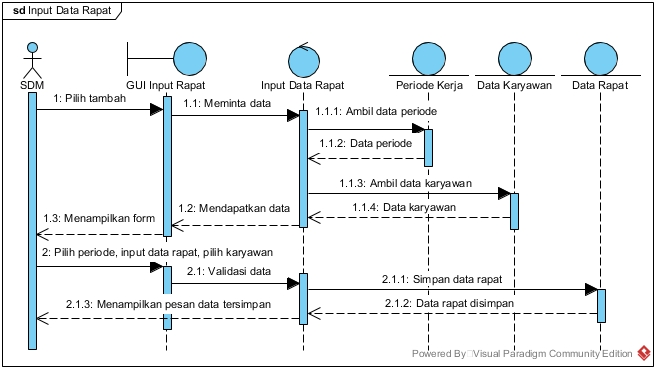
\includegraphics[width=14cm]{gambar/sequence/input-data-rapat}
            		    \caption{\emph{Sequence Diagram} Input Data Rapat}
            		    \label{sequence_input_rapat}
            		\end{figure}
            		\emph{Sequence Diagram} pada Gambar \ref{sequence_input_rapat} menjelaskan bagaimana urutan proses SDM melakukan \emph{input} data rapat karyawan. Langkah pertama adalah SDM memilih tambah data rapat, dan sistem akan mengambil data periode kerja dan data karyawan dari \emph{database} untuk ditampilkan pada \emph{form} tambah data rapat. Pada form tersebut SDM dapat memilih periode kerja dimana rapat tersebut dilaksanakan, memilih karyawan selaku peserta rapat dan data rapat lainnya. Sebelum data disimpan ke dalam \emph{database}, sistem akan melakukan validasi data terlebih dahulu. Kemudian sistem akan menampilkan pesan data tersimpan apabila data berhasil disimpan ke dalam \emph{database} Data Rapat. \newpage
            	    \item Rekap Upah Rapat
            	    \begin{figure}[H]
            		    \centering
            		    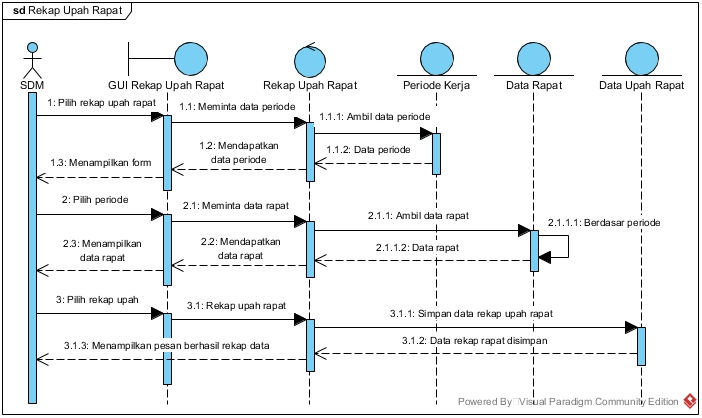
\includegraphics[width=13cm]{gambar/sequence/rekap-upah-rapat}
            		    \caption{\emph{Sequence Diagram} Rekap Upah Rapat}
            		    \label{sequence_upah_rapat}
            		\end{figure}
            		\emph{Sequence Diagram} pada Gambar \ref{sequence_upah_rapat} menjelaskan bagaimana urutan proses SDM melakukan perekapan upah rapat karyawan. Pertama SDM memilih rekap upah rapat dan sistem akan mengambil data periode kerja untuk ditampilkan dalam \emph{form}. SDM memilih periode kerja, kemudian sistem akan menampilkan data rapat karyawan selama periode yang dipilih. Setelah itu SDM dapat memilih rekap upah rapat karyawan sesuai data yang telah ditampilkan. Sistem akan melakukan perekapan upah rapat dan menyimpannya ke dalam \emph{database} data upah rapat. \newpage
            	    \item Lihat Data Rapat
            	    \begin{figure}[H]
            		    \centering
            		    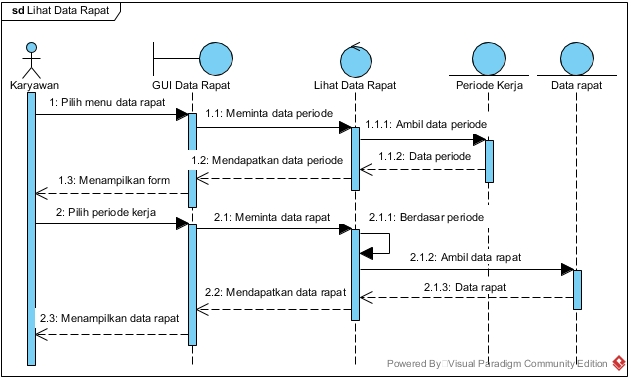
\includegraphics[width=13cm]{gambar/sequence/lihat-data-rapat}
            		    \caption{\emph{Sequence Diagram} Lihat Data Rapat}
            		    \label{sequence_lihat_rapat}
            		\end{figure}
            		\emph{Sequence Diagram} pada Gambar \ref{sequence_lihat_rapat} menjelaskan bagaimana urutan proses Karyawan melihat data rapat yang dihadiri oleh karyawan tersebut. Karyawan memilih lihat data rapat dan sistem akan mengambil data periode kerja dari dalam \emph{database} untuk ditampilkan pada \emph{form}. Setelah itu karyawan dapat memilih periode kerja sebagai parameter. Kemudian sistem mengambil data rapat berdasarkan periode kerja yang telah dipilih sebelumnya.
            	\end{enumerate}
			        
            	\item \emph{Sequence Diagram} Manajemen Data Lembur
            	
            	Dalam urutan proses manajemen data lembur terdapat terdapat beberapa \emph{sequence diagram} meliputi input data lembur, rekap upah lembur dan lihat data lembur. Detail dari masing-masing \emph{sequence} tersebut adalah sebagai berikut: \newpage
            	\begin{enumerate}[label=\alph*.]
            	    \itemsep0em
            	    \item Input Data Lembur
            	    \begin{figure}[H]
            		    \centering            		    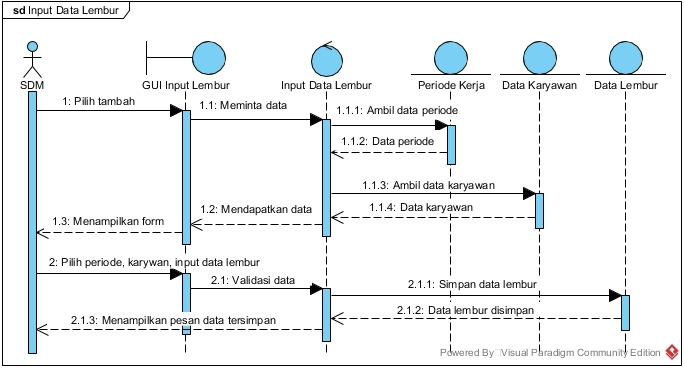
\includegraphics[width=14cm]{gambar/sequence/input-data-lembur}
            		    \caption{\emph{Sequence Diagram} Input Data Lembur}
            		    \label{sequence_input_lembur}
            		\end{figure}
            		\emph{Sequence Diagram} pada Gambar \ref{sequence_input_lembur} menjelaskan bagaimana urutan proses SDM melakukan \emph{input} data lembur karyawan. Langkah pertama adalah SDM memilih tambah data lembur, dan sistem akan mengambil data periode kerja dan data karyawan dari \emph{database} untuk ditampilkan pada \emph{form}. Pada form tersebut SDM dapat memilih periode kerja dimana lembur karyawan tersebut dilaksanakan, memilih karyawan yang lembur dan data lembur lainnya. Sebelum data disimpan ke dalam \emph{database}, sistem akan melakukan validasi data terlebih dahulu. Kemudian sistem akan menampilkan pesan data tersimpan apabila data berhasil disimpan ke dalam \emph{database} Data Lembur. \newpage
            	    \item Rekap Upah Lembur
            	    
            	    \emph{Sequence Diagram} yang menjelaskan urutan proses rekap upah lembur karyawan tidak jauh berbeda dengan urutan proses rekap upah rapat. Yang berbeda yaitu entitas yang digunakan adalah data lembur karyawan.
            	    \item Lihat Data Lembur
            	    \begin{figure}[H]
            		    \centering            		    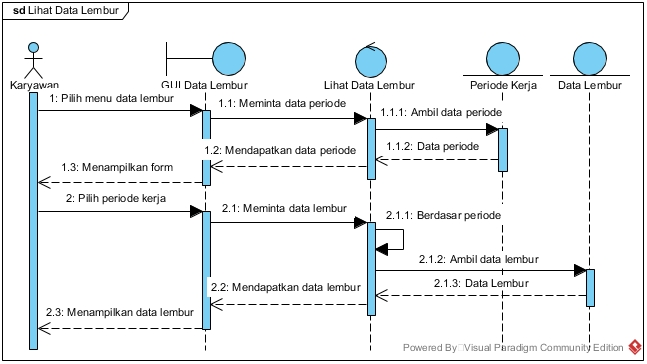
\includegraphics[width=13cm]{gambar/sequence/lihat-data-lembur}
            		    \caption{\emph{Sequence Diagram} Lihat Data Lembur}
            		    \label{sequence_lihat_lembur}
            		\end{figure}
            		\emph{Sequence Diagram} pada Gambar \ref{sequence_lihat_lembur} menjelaskan bagaimana urutan proses karyawan melihat data lembur. Langkah pertama karyawan memilih lihat data lembur dan sistem akan mengambil data periode kerja dari dalam \emph{database} untuk ditampilkan pada \emph{form}. Kemudian karyawan dapat memilih periode kerja sebagai parameter inputan. Setelah itu sistem mengambil data lembur karyawan berdasarkan periode kerja yang telah dipilih sebelumnya. \newpage
            	\end{enumerate}
			        
            	\item \emph{Sequence Diagram} Manajemen Data Absensi
            	
            	Dalam urutan proses manajemen data absensi karyawan terdapat terdapat beberapa \emph{sequence diagram} meliputi \emph{upload} data absensi, ubah data absensi dan lihat rekap absensi. Detail dari masing-masing \emph{sequence} tersebut adalah sebagai berikut:
            	\begin{enumerate}[label=\alph*.]
            	    \itemsep0em
            	    \item \emph{Upload} Data Absensi
            	    \begin{figure}[H]
            		    \centering            		    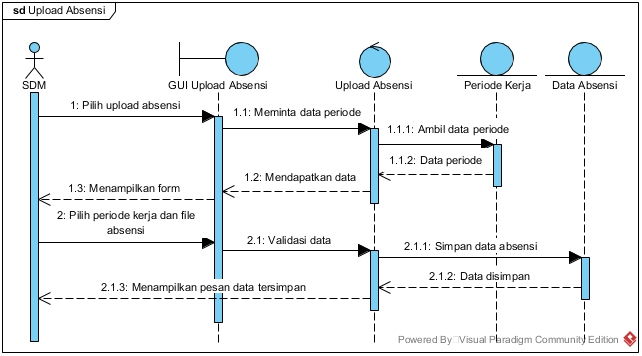
\includegraphics[width=13cm]{gambar/sequence/upload-data-absensi}
            		    \caption{\emph{Sequence Diagram} Upload Absensi}
            		    \label{sequence_upload_absensi}
            		\end{figure}
            		\emph{Sequence Diagram} pada Gambar \ref{sequence_upload_absensi} menjelaskan bagaimana urutan proses SDM melakukan \emph{upload} data absensi ke dalam sistem. Langkah pertama adalah SDM memilih tindakan \emph{upload} absensi, dan sistem akan mengambil data periode kerja dari \emph{database} untuk ditampilkan pada \emph{form upload} absensi. Pada \emph{form} tersebut SDM memilih periode kerja dari absensi dan memilih \emph{file} absensi. Sistem akan melakukan validasi data terlebih dahulu sebelum disimpan ke dalam \emph{database}. Kemudian sistem akan menampilkan pesan data tersimpan apabila data berhasil disimpan ke dalam \emph{database} Data Absensi. \newpage
            	    \item Lihat Rekap Absensi
            	    \begin{figure}[H]
            		    \centering
            		    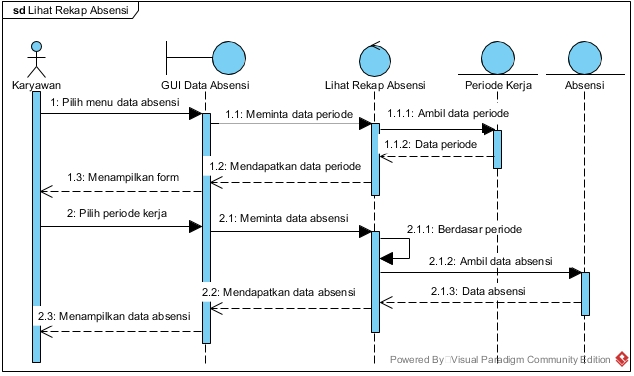
\includegraphics[width=13cm]{gambar/sequence/lihat-rekap-absensi}
            		    \caption{\emph{Sequence Diagram} Lihat Rekap Absensi}
            		    \label{sequence_lihat_absensi}
            		\end{figure}
            		\emph{Sequence Diagram} pada Gambar \ref{sequence_lihat_absensi} menjelaskan bagaimana urutan proses karyawan melihat data rekap absensi. Pertama karyawan memilih lihat data absensi dan sistem akan mengambil data periode kerja dari dalam \emph{database} untuk ditampilkan pada \emph{form}. Setelah itu karyawan dapat memilih periode kerja sebagai parameter. Kemudian sistem mengambil data absensi karyawan tersebut berdasarkan periode kerja yang telah dipilih sebelumnya. \newpage
            	\end{enumerate}
			        
            	\item \emph{Sequence Diagram} Manajemen Data Ujian
            	
            	Dalam urutan proses manajemen data ujian terdapat terdapat beberapa \emph{sequence} meliputi input data ujian, pengawas dan korektor ujian, rekap upah pengawas dan korektor ujian, serta lihat data pengawas dan kotektor ujian. Detail dari masing-masing \emph{sequence} tersebut adalah sebagai berikut:
            	\begin{enumerate}[label=\alph*.]
            	    \itemsep0em
            	    \item Input Data Ujian
            	    \begin{figure}[H]
            		    \centering            		    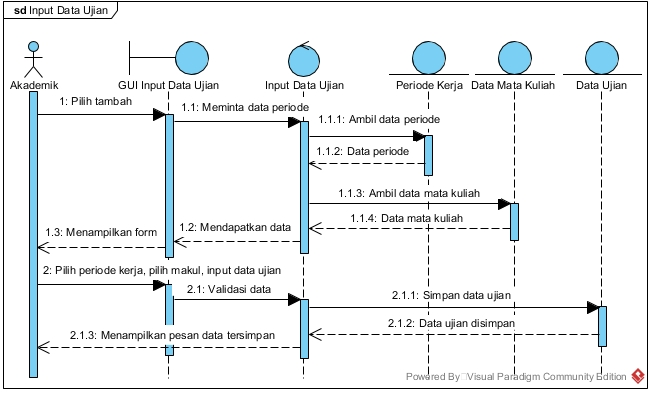
\includegraphics[width=13cm]{gambar/sequence/input-data-ujian}
            		    \caption{\emph{Sequence Diagram} Input Data Ujian}
            		    \label{sequence_input_ujian}
            		\end{figure}
            		\emph{Sequence Diagram} pada Gambar \ref{sequence_input_ujian} menjelaskan bagaimana urutan proses Akademik melakukan \emph{input} data ujian. Akademik memilih tambah data ujian, kemudian sistem akan mengambil data periode kerja dan data mata kuliah dari dalam \emph{database} untuk ditampilkan pada \emph{form} tambah data. Pada \emph{form} tersebut Akademik memilih periode kerja, mata kuliah ujian dan data ujian lainnya. Kemudian sistem akan melakukan validasi data sebelum disimpan ke dalam \emph{database}. Terakhir sistem akan menampilkan pesan data tersimpan apabila data berhasil disimpan ke dalam \emph{database} Data Ujian. \newpage
            	    \item Input Data Pengawas Ujian
            	    \begin{figure}[H]
            		    \centering
            		    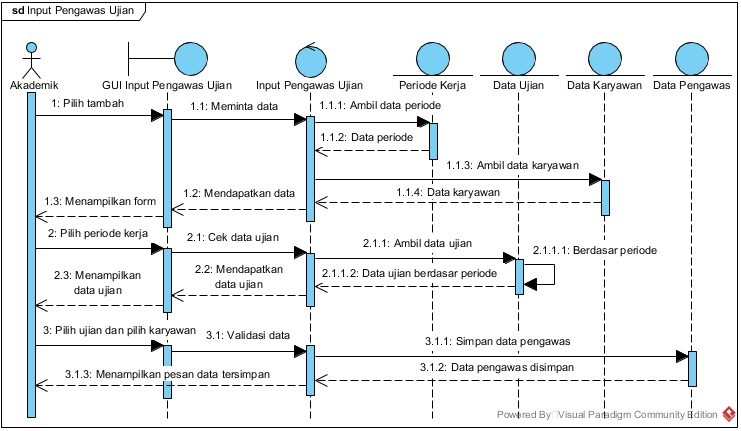
\includegraphics[width=14cm]{gambar/sequence/input-data-pengawas}
            		    \caption{\emph{Sequence Diagram} Input Data Pengawas Ujian}
            		    \label{sequence_input_pengawas}
            		\end{figure}
            		\emph{Sequence Diagram} pada Gambar \ref{sequence_input_pengawas} menjelaskan bagaimana urutan proses Akademik mengisi data pengawas ujian. Pertama Akademik memilih tambah data pengawas dan sistem akan mengambil data periode kerja dari dalam \emph{database} untuk ditampilkan pada \emph{form}. Pada \emph{form} tersebut Akademik akan memilih periode kerja, kemudian sistem akan mengambil data ujian sesuai periode kerja yang dipilih dan ditampilkan dalam \emph{form}. Setelah itu Akademik memilih ujian dan karyawan yang menjadi pengawas ujian tersebut. Sistem akan melakukan validasi sebelum data disimpan. Terakhir sistem akan menampilkan pesan data tersimpan apabila data berhasil disimpan ke dalam \emph{database} Pengawas Ujian. \newpage
            	    \item Input Data Korektor Ujian
            	    \begin{figure}[H]
            		    \centering
            		    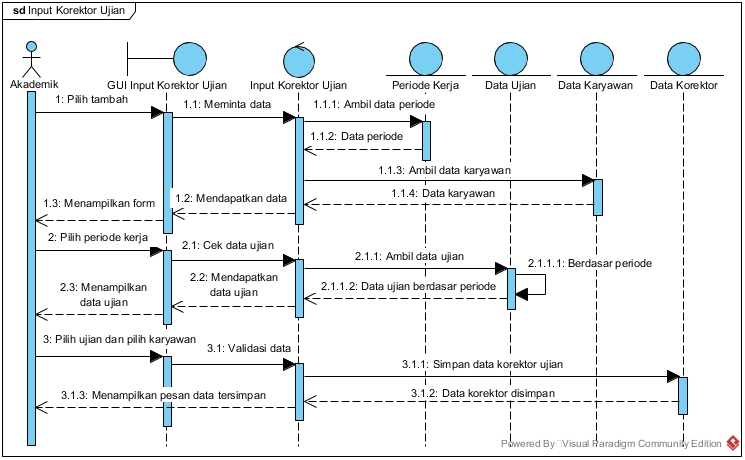
\includegraphics[width=14cm]{gambar/sequence/input-data-korektor}
            		    \caption{\emph{Sequence Diagram} Input Data Korektor Ujian}
            		    \label{sequence_input_korektor}
            		\end{figure}
            		\emph{Sequence Diagram} pada Gambar \ref{sequence_input_korektor} menjelaskan bagaimana urutan proses Akademik mengisi data korektor ujian. Pertama Akademik memilih tambah data korektor dan sistem akan mengambil data periode kerja dari dalam \emph{database} untuk ditampilkan pada \emph{form}. Pada \emph{form} tersebut Akademik akan memilih periode kerja, kemudian sistem akan mengambil data ujian sesuai periode kerja yang dipilih dan ditampilkan dalam \emph{form}. Setelah itu Akademik memilih ujian dan karyawan yang menjadi korektor ujian tersebut. Sistem akan melakukan validasi sebelum data disimpan. Terakhir sistem akan menampilkan pesan data tersimpan apabila data berhasil disimpan ke dalam \emph{database} Korektor Ujian. \newpage
            	    \item Lihat Data Pengawas Ujian
            	    \begin{figure}[H]
            		    \centering
            		    \includegraphics[width=13cm]{gambar/sequence/lihat-data-pengawas}
            		    \caption{\emph{Sequence Diagram} Lihat Data Pengawas Ujian}
            		    \label{sequence_lihat_pengawas}
            		\end{figure}
            		\emph{Sequence Diagram} pada Gambar \ref{sequence_lihat_pengawas} menjelaskan bagaimana urutan proses karyawan melihat data pengawas ujian. Langkah pertama karyawan memilih lihat data pengawas ujian dan sistem akan mengambil data periode kerja dari dalam \emph{database} untuk ditampilkan pada \emph{form}. Setelah itu karyawan dapat memilih periode kerja sebagai parameter. Kemudian sistem mengambil data pengawas ujian yang dilakukan oleh karyawan berdasarkan periode kerja yang telah dipilih sebelumnya.
            	    \item Lihat Data Korektor Ujian
            	    
            	    \emph{Sequence Diagram} untuk lihat data korektor ujian tidak jauh berbeda dengan lihat data pengawas ujian, hanya saja entitas yang digunakan adalah data korektor ujian.
            	    \item Rekap Upah Pengawas dan Korektor Ujian
            	    
            	    \emph{Sequence Diagram} untuk urutan proses rekap upah pengawas dan korektor ujian juga tidak jauh berbeda dengan urutan proses rekap upah rapat ataupun lembur.
            	\end{enumerate}
            	    
            	\item \emph{Sequence Diagram} Manajemen Laporan Kerja Karyawan
            	
            	Dalam urutan proses manajamen data laporan kerja karyawan terdapat beberapa \emph{sequence} meliputi input rencana kerja dan laporan harian, input checklist dan laporan bulanan, serta lihat data laporan kerja. Penjelasan dari masing-masing \emph{sequence} adalah sebagai berikut:
            	\begin{enumerate}[label=\alph*.]
            	    \itemsep0em
            	    \item Input Rencana Kerja Harian
            	    \begin{figure}[H]
            		    \centering            		    \includegraphics[width=14cm]{gambar/sequence/input-propeka-rkh}
            		    \caption{\emph{Sequence Diagram} Input Rencana Kerja Harian}
            		    \label{sequence_input_propeka_rkh}
            		\end{figure}
            		\emph{Sequence Diagram} pada Gambar \ref{sequence_input_propeka_rkh} menjelaskan bagaimana urutan proses karyawan melakukan input data rencana kerja harian (RKH). Pada \emph{form} tambah data RKH, karyawan memilih periode kerja dan tanggal. Sistem kemudian akan melakukan pengecekan apakah data RKH untuk periode dan tanggal yang dipilih sudah ada atau belum. Apabila sudah ada maka sistem akan menampilkan pesan bahwa RKH untuk periode dan tanggal yang dipilih sudah diisi. Sedangkan apabila data belum ada, karyawan dapat melakukan pengisian data RKH berupa rencana kegiatan-kegiatan selama satu hari.
            	    \item Input Laporan Kerja Harian
            	    \begin{figure}[H]
            		    \centering            		    \includegraphics[width=14cm]{gambar/sequence/input-propeka-lh}
            		    \caption{\emph{Sequence Diagram} Input Laporan Kerja Harian}
            		    \label{sequence_input_propeka_lh}
            		\end{figure}
            		\emph{Sequence Diagram} pada Gambar \ref{sequence_input_propeka_lh} menjelaskan bagaimana urutan proses karyawan melakukan input data laporan kerja harian (LH). Karyawan terlebih dahulu memilih periode kerja dan tanggal. Kemudian sistem akan mengecek ketersediaan data RKH dalam \emph{database}. Apabila data RKH tidak ada, maka sistem akan menampilkan pesan bahwa RKH untuk tanggal yang dipilih belum dibuat. Sedangkan apabila data RKH sudah ada, sistem akan menampilkan kegiatan-kegiatan RKH beserta \emph{form} untuk mengisi data LH.
            	    \item Input Checklist Bulanan
            	    \begin{figure}[H]
            		    \centering            		    \includegraphics[width=14cm]{gambar/sequence/input-propeka-cb}
            		    \caption{\emph{Sequence Diagram} Input Checklist Bulanan}
            		    \label{sequence_input_propeka_cb}
            		\end{figure}
            		\emph{Sequence Diagram} pada Gambar \ref{sequence_input_propeka_cb} menjelaskan bagaimana urutan proses karyawan melakukan input data rencana kerja bulanan atau biasa disebut checklist bulanan (CB). Pada \emph{form} tambah data CB, karyawan harus memilih periode kerja terlebih dahulu sebagai parameter. Sistem kemudian akan melakukan pengecekan apakah data CB untuk periode yang dipilih sudah ada atau belum. Apabila sudah ada maka sistem akan menampilkan pesan bahwa CB untuk periode yang dipilih sudah diisi. Sedangkan apabila data belum ada, karyawan dapat melakukan pengisian data CB berupa rencana kegiatan-kegiatan selama satu periode kerja.
            	    \item Input Laporan Kerja Bulanan
            	    \begin{figure}[H]
            		    \centering            		    \includegraphics[width=14cm]{gambar/sequence/input-propeka-lb}
            		    \caption{\emph{Sequence Diagram} Input Laporan Kerja Bulanan}
            		    \label{sequence_input_propeka_lb}
            		\end{figure}
            		\emph{Sequence Diagram} pada Gambar \ref{sequence_input_propeka_lb} menjelaskan bagaimana urutan proses karyawan melakukan input data laporan kerja bulanan (LB). Karyawan terlebih dahulu memilih periode kerja sebagai parameter. Kemudian sistem akan mengecek ketersediaan data checklist bulanan (CB) dalam \emph{database}. Apabila data CB tidak ada, maka sistem akan menampilkan pesan bahwa CB untuk periode kerja yang dipilih belum dibuat. Sedangkan apabila data CB sudah ada, sistem akan menampilkan kegiatan-kegiatan CB beserta \emph{form} untuk mengisi data LB.
            	\end{enumerate}
            	\newpage
            	\item \emph{Sequence Diagram} Manajemen Penilaian Kinerja Karyawan
            	
            	Proses manajemen penilaian kinerja karyawan ini memiliki beberapa \emph{sequence} yang meliputi input penilaian kinerja dan lihat data penilaian kinerja. Detail dari masing-masing \emph{sequence} tersebut adalah sebagai berikut:
            	\begin{enumerate}[label=\alph*.]
            	    \itemsep0em
            	    \item Input Penilaian Kinerja
            	    \begin{figure}[H]
            		    \centering
            		    \includegraphics[width=14cm]{gambar/sequence/input-penilaian-kinerja}
            		    \caption{\emph{Sequence Diagram} Input Penilaian Kinerja Karyawan}
            		    \label{sequence_input_penilaian}
            		\end{figure}
            		\emph{Sequence Diagram} pada Gambar \ref{sequence_input_penilaian} menjelaskan bagaimana urutan proses Kepala Unit mengisi data penilaian kinerja karyawan yang dibawahinya. Pada halaman penilaian kinerja, Kepala Unit memilih input penilaian dan sistem akan mengambil data periode kerja dan data karyawan untuk ditampilkan ke dalam \emph{form} penilaian. Setelah itu Kepala Unit memilih periode kerja dan mengisi penilaian kinerja karyawan. Kemudian sistem akan melakukan validasi data tersebut sebelum disimpan ke dalam \emph{database}. Sistem akan menampilkan pesan data tersimpan apabila data berhasil disimpan. \newpage
            	    \item Lihat Data Penilaian Kinerja
            	    \begin{figure}[H]
            		    \centering
            		    \includegraphics[width=13cm]{gambar/sequence/lihat-data-penilaian}
            		    \caption{\emph{Sequence Diagram} Lihat Data Penilaian Kinerja}
            		    \label{sequence_lihat_penilaian}
            		\end{figure}
            		\emph{Sequence Diagram} pada Gambar \ref{sequence_lihat_penilaian} menjelaskan bagaimana urutan proses karyawan melihat data penilaian kinerja. Pertama karyawan memilih lihat data penilaian dan sistem akan mengambil data periode kerja dari dalam \emph{database} untuk ditampilkan pada \emph{form}. Setelah itu karyawan dapat memilih periode kerja sebagai parameter. Kemudian sistem mengambil data penilaian kinerja karyawan tersebut berdasarkan periode kerja yang telah dipilih sebelumnya. \newpage
            	\end{enumerate}
			        
            	\item \emph{Sequence Diagram} Input Insentif Operasional
            	    \begin{figure}[H]
            		    \centering
            		    \includegraphics[width=14cm]{gambar/sequence/input-insentif-operasional}
            		    \caption{\emph{Sequence Diagram} Input Insentif Operasional}
            		    \label{sequence_input_insentif}
            		\end{figure}
            		\emph{Sequence Diagram} pada Gambar \ref{sequence_input_insentif} menjelaskan bagaimana urutan proses Kepala Unit mengisi data insentif operasional karyawan yang dibawahinya. Pada halaman insentif operasional, Kepala Unit memilih tambah insentif operasional dan sistem akan mengambil data periode kerja dan data karyawan untuk ditampilkan ke dalam \emph{form} input insentif operasional. Setelah itu Kepala Unit memilih periode kerja dan mengisi data insentif operasional karyawan. Kemudian sistem akan melakukan validasi data tersebut sebelum disimpan ke dalam \emph{database}. Sistem akan menampilkan pesan data tersimpan apabila data berhasil disimpan. \newpage
			        
            	\item \emph{Sequence Diagram Generate} Slip Gaji
			        \begin{figure}[H]
            		    \centering            		    \includegraphics[width=14cm]{gambar/sequence/generate-slip-gaji}
            		    \caption{\emph{Sequence Diagram Generate} Slip Gaji}
            		    \label{sequence_generate_slip}
            		\end{figure}
            		\emph{Sequence Diagram} pada Gambar \ref{sequence_generate_slip} menjelaskan bagaimana urutan proses staf Keuangan melakukan \emph{generate} slip gaji karyawan. Pertama sistem akan mengambil data periode kerja dan data unit kerja untuk ditampilkan dalam \emph{form}. Kemudian staf Keuangan memilih periode kerja dan unit kerja sebagai parameter. Sistem akan mengambil data upah karyawan berdasarkan periode kerja dan unit kerja yang dipilih, dan melakukan kalkulasi upah karyawan tersebut. Lalu sistem akan menampilkannya kepada staf Keuangan. Setelah itu staf Keuangan memilih \emph{generate} slip gaji dan sistem akan melakukan proses \emph{generate} slip dan menyimpannya ke dalam \emph{database}.
            		\newpage
            	\item \emph{Sequence Diagram} Cetak Slip Gaji
			        \begin{figure}[H]
            		    \centering            		    \includegraphics[width=12cm]{gambar/sequence/cetak-slip-gaji}
            		    \caption{\emph{Sequence Diagram} Cetak Slip Gaji}
            		    \label{sequence_cetak_slip}
            		\end{figure}
            		\emph{Sequence Diagram} pada Gambar \ref{sequence_cetak_slip} menjelaskan bagaimana urutan proses karyawan melakukan cetak slip gaji. Karyawan memilih periode kerja dan sistem akan mengambil data slip gaji karyawan berdasarkan periode yang dipilih. Kemudian sistem menampilkan data slip gaji tersebut kepada karyawan. Setelah itu karyawan memilih cetak slip gaji, dan sistem akan melakukan \emph{export} data slip gaji tersebut.
			\end{enumerate}
			
			\subsubsection{\emph{Entity Relationship Diagram}}
			Peneliti selanjutnya membuat ERD dengan tujuan untuk menjelaskan keterkaitan antara data satu dengan yang lainnya. Berdasarkan ERD pada Gambar \ref{erd_penggajian}, nantinya akan diketahui secara garis besar tabel apa saja yang dibutuhkan oleh sistem yang dikembangkan.
			\newpage
			\begin{figure}[H]
			    \centering
			    \includegraphics[width=14cm]{gambar/entity/ERD-versi3}
			    \caption{ERD Sistem Informasi Penggajian Karyawan}
			    \label{erd_penggajian}
			\end{figure}

		\subsection{Perancangan Basis Data}
		Perancangan basis data merupakan rancangan struktur tabel yang nantinya akan menjadi basis data dari sistem yang dikembangkan.
		
		    \subsubsection{Hasil Rancangan Basis Data}
		    Berikut merupakan hasil dari perancangan basis data pada sistem yang dikembangkan:
		    \begin{enumerate}
		        \itemsep0em
			    \item Tabel Bidang Kerja (\texttt{master\_bidang})
		        
		        Tabel Bidang Kerja berfungsi untuk menyimpan data bidang kerja. Selanjutnya tabel tersebut diberi nama \texttt{master\_bidang}. Detail dari tabel tersebut dapat dilihat pada Tabel \ref{tabel_bidang}.
		        \begin{spacing}{1.0}
		        \begin{longtable}{|>{\centering}p{1.5em}|p{3cm}|p{3cm}|p{3cm}|p{2cm}|}
			        \caption{Tabel Bidang Kerja (\texttt{master\_bidang})} \label{tabel_bidang} \\
                    \hline \textbf{No.} & \textbf{Colomn} & \textbf{Type} & \textbf{Constraint} & \textbf{Extra}  \\ \hline 
                    \endfirsthead
                    \multicolumn{5}{c}%
                    {{\bfseries \tablename\ \thetable{}: }Tabel Bidang Kerja (\texttt{master\_bidang}) (lanjutan)} \\
                    \hline \textbf{No.} & \textbf{Colomn} & \textbf{Type} & \textbf{Constraint} & \textbf{Extra}  \\ \hline
                    \endhead
                    \hline
                    \hline \hline
                    \endlastfoot
                    
                    1. & kode\_bidang & character varying(10) & PRIMARY KEY, NOT NULL & \\ \hline
                    2. & nama\_bidang & character varying(30) & NOT NULL & \\ \hline
                    3. & keterangan & character varying(50) & & \\ \hline
			    \end{longtable}
			    \end{spacing}
			    \vspace{4mm}
		        \item Tabel Unit Kerja (\texttt{master\_unit\_kerja})
		        
		        Tabel Unit Kerja berfungsi untuk menyimpan data unit kerja. Selanjutnya tabel tersebut diberi nama \texttt{master\_unit\_kerja}. Detail dari tabel tersebut dapat dilihat pada Tabel \ref{tabel_unit_kerja}.
		        \begin{spacing}{1.0}
		        \begin{longtable}{|>{\centering}p{1.5em}|p{3cm}|p{3cm}|p{3cm}|p{2cm}|}
			        \caption{Tabel Unit Kerja (\texttt{master\_unit\_kerja})} \label{tabel_unit_kerja} \\
                    \hline \textbf{No.} & \textbf{Colomn} & \textbf{Type} & \textbf{Constraint} & \textbf{Extra}  \\ \hline 
                    \endfirsthead
                    \multicolumn{5}{c}%
                    {{\bfseries \tablename\ \thetable{}: }Tabel Unit Kerja (\texttt{master\_unit\_kerja}) (lanjutan)} \\
                    \hline \textbf{No.} & \textbf{Colomn} & \textbf{Type} & \textbf{Constraint} & \textbf{Extra}  \\ \hline
                    \endhead
                    \hline
                    \endfoot
                    \hline \hline
                    \endlastfoot
                    
                    1. & kode\_unit & character varying(20) & PRIMARY KEY, NOT NULL & \\ \hline
                    2. & kode\_bidang & character varying(10) & NOT NULL & \\ \hline
                    3. & nama\_unit & character varying(50) & & \\ \hline
                    4. & keterangan & character varying(50) & & \\ \hline
			    \end{longtable}
			    \end{spacing}
			    \vspace{4mm}
		        \item Tabel Jabatan (\texttt{master\_jabatan})
		        
		        Tabel Jabatan berfungsi untuk menyimpan data master jabatan yang ada di Universitas Proklamasi 45 Yogyakarta. Selanjutnya tabel tersebut diberi nama \texttt{master\_jabatan}. Detail dari tabel master jabatan dapat dilihat pada Tabel \ref{tabel_jabatan}.
		        \begin{spacing}{1.0}
		        \begin{longtable}{|>{\centering}p{1.5em}|p{3cm}|p{3cm}|p{3cm}|p{2cm}|}
			        \caption{Tabel Jabatan (\texttt{master\_jabatan})} \label{tabel_jabatan} \\
                    \hline \textbf{No.} & \textbf{Colomn} & \textbf{Type} & \textbf{Constraint} & \textbf{Extra}  \\ \hline 
                    \endfirsthead
                    \multicolumn{5}{c}%
                    {{\bfseries \tablename\ \thetable{}: }Tabel Jabatan (\texttt{master\_jabatan}) (lanjutan)} \\
                    \hline \textbf{No.} & \textbf{Colomn} & \textbf{Type} & \textbf{Constraint} & \textbf{Extra}  \\ \hline
                    \endhead
                    \hline
                    \endfoot
                    \hline \hline
                    \endlastfoot
                    
                    1. & kode\_jabatan & character varying(20) & PRIMARY KEY, NOT NULL & \\ \hline
                    2. & nama\_jabatan & character varying(50) & NOT NULL & \\ \hline
                    3. & tunjangan\_jabatan & integer & NOT NULL & default: 0 \\ \hline
                    4. & keterangan & character varying(50) & & \\ \hline
                    5. & under\_of\_jabatan & character varying(20) & NOT NULL & \\ \hline
                    6. & max\_satu & enum (ya,tidak) &  & default: ya \\ \hline
                    7. & tersedia & enum (ya,tidak) & & default: ya \\ \hline
                    
			    \end{longtable}
			    \end{spacing}
			    \vspace{4mm}
			    \newpage
		        \item Tabel Periode Kerja (\texttt{master\_periode})
		        
		        Tabel periode kerja berfungsi untuk menyimpan data master periode kerja. Selanjutnya tabel tersebut diberi nama \texttt{master\_periode}. Detail dari tabel periode kerja dapat dilihat pada Tabel \ref{tabel_periode}.
		        \begin{spacing}{1.0}
		        \begin{longtable}{|>{\centering}p{1.5em}|p{3cm}|p{3cm}|p{3cm}|p{2cm}|}
			        \caption{Tabel Periode Kerja (\texttt{master\_periode})} \label{tabel_periode} \\
                    \hline \textbf{No.} & \textbf{Colomn} & \textbf{Type} & \textbf{Constraint} & \textbf{Extra}  \\ \hline 
                    \endfirsthead
                    \multicolumn{5}{c}%
                    {{\bfseries \tablename\ \thetable{}: }Tabel Periode Kerja (\texttt{master\_periode}) (lanjutan)} \\
                    \hline \textbf{No.} & \textbf{Colomn} & \textbf{Type} & \textbf{Constraint} & \textbf{Extra}  \\ \hline
                    \endhead
                    \hline
                    \endfoot
                    \hline \hline
                    \endlastfoot
                    
                    1. & id\_periode & integer & PRIMARY KEY, NOT NULL & Auto Increment \\ \hline
                    2. & tahun & year(4) & NOT NULL & \\ \hline
                    3. & bulan & character varying(15) & NOT NULL & \\ \hline
                    4. & mulai & date & NOT NULL & \\ \hline
                    5. & akhir & date & NOT NULL & \\ \hline
                    6. & hari\_aktif & integer & NOT NULL & \\ \hline
                    7. & pembagi & float & NOT NULL & \\ \hline
                    8. & aktif & enum (ya,tidak) & & default: tidak \\ \hline
			    \end{longtable}
			    \end{spacing}
			    \vspace{4mm}
			    \item Tabel Jam Kerja (\texttt{master\_jam\_kerja})
			    
			    Tabel jam kerja berfungsi untuk menyimpan data master jam kerja karyawan. Selanjutnya tabel tersebut diberi nama \texttt{master\_jam\_kerja}. Detail dari tabel jam kerja dapat dilihat pada Tabel \ref{tabel_jam_kerja}.
			    \begin{spacing}{1.0}
		        \begin{longtable}{|>{\centering}p{1.5em}|p{3.5cm}|p{2.5cm}|p{3cm}|p{2cm}|}
			        \caption{Tabel Jam Kerja (\texttt{master\_jam\_kerja})} \label{tabel_jam_kerja} \\
                    \hline \textbf{No.} & \textbf{Colomn} & \textbf{Type} & \textbf{Constraint} & \textbf{Extra}  \\ \hline 
                    \endfirsthead
                    \multicolumn{5}{c}%
                    {{\bfseries \tablename\ \thetable{}: }Tabel Jam Kerja (\texttt{master\_jam\_kerja}) (lanjutan)} \\
                    \hline \textbf{No.} & \textbf{Colomn} & \textbf{Type} & \textbf{Constraint} & \textbf{Extra}  \\ \hline
                    \endhead
                    \hline
                    \endfoot
                    \hline \hline
                    \endlastfoot
                    
                    1. & kode\_jam\_kerja & character varying(20) & PRIMARY KEY, NOT NULL & \\ \hline
                    2. & nama\_jam\_kerja & character varying(30) & NOT NULL & \\ \hline
                    3. & jumlah\_jam & integer & NOT NULL & \\ \hline
                    4. & jam\_datang & time & NOT NULL & \\ \hline
                    5. & jam\_pulang & time & NOT NULL & \\ \hline
                    6. & jam\_istirahat & time & NOT NULL & \\ \hline
                    7. & toleransi & time & NOT NULL & \\ \hline
                    8. & jam\_datang\_sabtu & time & NOT NULL & \\ \hline
                    9. & jam\_pulang\_sabtu & time & NOT NULL & \\ \hline
                    10. & jam\_istirahat\_sabtu & time & NOT NULL & \\ \hline
                    11. & toleransi\_sabtu & time & NOT NULL & \\ \hline
			    \end{longtable}
			    \end{spacing}
			    \vspace{4mm}
		        \item Tabel Nominal (\texttt{master\_nominal})
		        
		        Tabel nominal berfungsi untuk menyimpan data master besaran nominal upah dan juga potongan yang termasuk komponen penggajian. Selanjutnya tabel tersebut diberi nama \texttt{master\_nominal}. Detail dari tabel nominal dapat dilihat pada Tabel \ref{tabel_nominal}.
		        \begin{spacing}{1.0}
		        \begin{longtable}{|>{\centering}p{1.5em}|p{3cm}|p{3cm}|p{3cm}|p{2cm}|}
			        \caption{Tabel Nominal (\texttt{master\_nominal})} \label{tabel_nominal} \\
                    \hline \textbf{No.} & \textbf{Colomn} & \textbf{Type} & \textbf{Constraint} & \textbf{Extra}  \\ \hline 
                    \endfirsthead
                    \multicolumn{5}{c}%
                    {{\bfseries \tablename\ \thetable{}: }Tabel Nominal (\texttt{master\_nominal}) (lanjutan)} \\
                    \hline \textbf{No.} & \textbf{Colomn} & \textbf{Type} & \textbf{Constraint} & \textbf{Extra}  \\ \hline
                    \endhead
                    \hline
                    \endfoot
                    \hline \hline
                    \endlastfoot
                    
                    1. & id\_nominal & integer & PRIMARY KEY, NOT NULL & Auto Increment \\ \hline
                    2. & tpd & integer & NOT NULL & \\ \hline
                    3. & lembur & integer & NOT NULL & \\ \hline
                    4. & uang\_makan & integer & NOT NULL & \\ \hline
                    5. & rapat & integer & NOT NULL & \\ \hline
                    6. & transport\_reguler & integer & NOT NULL & \\ \hline
                    7. & transport\_malam & integer & NOT NULL & \\ \hline
                    8. & sks & integer & NOT NULL & \\ \hline
                    9. & tunjangan\_bpjs & integer & NOT NULL & \\ \hline
                    10. & potongan\_bpjs & integer & NOT NULL & \\ \hline
                    11. & potongan\_koperasi & integer & NOT NULL & \\ \hline
                    12. & hal\_khusus & integer & NOT NULL & \\ \hline
                    13. & korektor\_ujian & integer & NOT NULL & \\ \hline
                    14. & pengawas\_reguler & integer & NOT NULL & \\ \hline
                    15. & pengawas\_malam & integer & NOT NULL & \\ \hline
                    16. & aktif & enum (ya,tidak) & & default: tidak \\ \hline
			    \end{longtable}
			    \end{spacing}
			    \vspace{4mm}
		        \item Tabel Program Studi (\texttt{master\_program\_studi})
		        
		        Tabel program studi berfungsi menyimpan data nama-nama program studi yang ada. Selanjutnya tabel tersebut diberi nama \texttt{master\_prodi}. Detail tabel program studi dapat dilihat pada Tabel \ref{tabel_prodi}.
		        \begin{spacing}{1.0}
		        \begin{longtable}{|>{\centering}p{1.5em}|p{3cm}|p{3cm}|p{3cm}|p{2cm}|}
			        \caption{Tabel Program Studi (\texttt{master\_prodi})} \label{tabel_prodi} \\
                    \hline \textbf{No.} & \textbf{Colomn} & \textbf{Type} & \textbf{Constraint} & \textbf{Extra}  \\ \hline 
                    \endfirsthead
                    \multicolumn{5}{c}%
                    {{\bfseries \tablename\ \thetable{}: }Tabel Program Studi (\texttt{master\_prodi}) (lanjutan)} \\
                    \hline \textbf{No.} & \textbf{Colomn} & \textbf{Type} & \textbf{Constraint} & \textbf{Extra}  \\ \hline
                    \endhead
                    \hline
                    \endfoot
                    \hline \hline
                    \endlastfoot
                    
                    1. & kode\_prodi & character varying(10) & PRIMARY KEY, NOT NULL & \\ \hline
                    2. & nama\_prodi & character varying(50) & NOT NULL & \\ \hline
                    3. & kode\_fakultas & character varying(20) & NOT NULL & \\ \hline
                    4. & keterangan & character varying(50) & & \\ \hline
			    \end{longtable}
			    \end{spacing}
			    \vspace{4mm}
		        \item Tabel Mata Kuliah (\texttt{master\_matakuliah})
		        
		        Tabel mata kuliah berfungsi menyimpan data nama-nama mata kuliah yang ada. Selanjutnya tabel tersebut diberi nama \texttt{master\_matakuliah}. Detail tabel mata kuliah dapat dilihat pada Tabel \ref{tabel_makul}.
		        \begin{spacing}{1.0}
		        \begin{longtable}{|>{\centering}p{1.5em}|p{3cm}|p{3cm}|p{3cm}|p{2cm}|}
			        \caption{Tabel Mata Kuliah (\texttt{master\_matakuliah})} \label{tabel_makul} \\
                    \hline \textbf{No.} & \textbf{Colomn} & \textbf{Type} & \textbf{Constraint} & \textbf{Extra}  \\ \hline 
                    \endfirsthead
                    \multicolumn{5}{c}%
                    {{\bfseries \tablename\ \thetable{}: }Tabel Mata Kuliah (\texttt{master\_matakuliah}) (lanjutan)} \\
                    \hline \textbf{No.} & \textbf{Colomn} & \textbf{Type} & \textbf{Constraint} & \textbf{Extra}  \\ \hline
                    \endhead
                    \hline
                    \endfoot
                    \hline \hline
                    \endlastfoot
                    
                    1. & kode\_matakuliah & character varying(10) & PRIMARY KEY, NOT NULL & \\ \hline
                    2. & nama\_matakuliah & character varying(50) & NOT NULL & \\ \hline
                    3. & sks\_matakuliah & integer & NOT NULL & \\ \hline
                    4. & smt\_matakuliah & integer & NOT NULL & \\ \hline
                    5. & kode\_prodi & character varying(10) & FOREIGN KEY, NOT NULL & \\ \hline
			    \end{longtable}
			    \end{spacing}
			    \vspace{4mm}
			    \item Tabel Karyawan (\texttt{data\_pegawai})
		        
		        Tabel Karyawan berfungsi untuk menyimpan data karyawan. Selanjutnya tabel tersebut diberi nama \texttt{data\_pegawai}. Detail dari tabel karyawan dapat dilihat pada Tabel \ref{tabel_karyawan}.
		        \begin{spacing}{1.0}
		        \begin{longtable}{|>{\centering}p{1.5em}|p{3cm}|p{3cm}|p{3cm}|p{2cm}|}
			        \caption{Tabel Karyawan (\texttt{data\_karyawan})} \label{tabel_karyawan} \\
                    \hline \textbf{No.} & \textbf{Colomn} & \textbf{Type} & \textbf{Constraint} & \textbf{Extra}  \\ \hline 
                    \endfirsthead
                    \multicolumn{5}{c}%
                    {{\bfseries \tablename\ \thetable{}: }Tabel Karyawan (\texttt{data\_karyawan}) (lanjutan)} \\
                    \hline \textbf{No.} & \textbf{Colomn} & \textbf{Type} & \textbf{Constraint} & \textbf{Extra}  \\ \hline
                    \endhead
                    \hline
                    \endfoot
                    \hline \hline
                    \endlastfoot
                    
                    1. & nip & character varying(30) & PRIMARY KEY, NOT NULL & \\ \hline
                    2. & nama & character varying(50) & NOT NULL & \\ \hline
                    3. & email & character varying(30) & & \\ \hline
                    4. & status\_karyawan & character varying(10) & & \\ \hline
                    5. & kode\_jam\_kerja & character varying(10) & FOREIGN KEY, NOT NULL & \\ \hline
                    6. & kode\_unit & character varying(20) & FOREIGN KEY, NOT NULL & \\ \hline
                    7. & kode\_jabatan & character varying(20) & FOREIGN KEY, NOT NULL & \\ \hline
                    8. & gaji\_pokok & integer & NOT NULL & \\ \hline
                    9. & tgppw & integer & NOT NULL & \\ \hline
                    10. & bpjs\_aktif & enum (ya,tidak) & & default: tidak \\ \hline
                    11. & koperasi\_aktif & enum (ya,tidak) & & default: tidak \\ \hline
                    12. & username & character varying(20) & NOT NULL & \\ \hline
                    13. & password & character varying(64) & NOT NULL & \\ \hline
			    \end{longtable}
			    \end{spacing}
			    \vspace{4mm}
		        \item Tabel Data Absensi (\texttt{absensi\_data})
		        
		        Tabel data absensi berfungsi menyimpan data absensi harian masing-masing karyawan. Selanjutnya tabel absensi tersebut diberi nama \texttt{absensi\_data}. Detail dari tabel absensi dapat dilihat pada Tabel \ref{tabel_absensi}.
		        \begin{spacing}{1.0}
		        \begin{longtable}{|>{\centering}p{1.5em}|p{3cm}|p{3cm}|p{3cm}|p{2cm}|}
			        \caption{Tabel Data Absensi (\texttt{absensi\_data})} \label{tabel_absensi} \\
                    \hline \textbf{No.} & \textbf{Colomn} & \textbf{Type} & \textbf{Constraint} & \textbf{Extra}  \\ \hline 
                    \endfirsthead
                    \multicolumn{5}{c}%
                    {{\bfseries \tablename\ \thetable{}: }Tabel Data Absensi (\texttt{absensi\_data}) (lanjutan)} \\
                    \hline \textbf{No.} & \textbf{Colomn} & \textbf{Type} & \textbf{Constraint} & \textbf{Extra}  \\ \hline
                    \endhead
                    \hline
                    \endfoot
                    \hline \hline
                    \endlastfoot
                    
                    1. & id\_absensi & integer & PRIMARY KEY, NOT NULL & Auto Increment \\ \hline
                    2. & id\_periode & integer & FOREIGN KEY, NOT NULL & \\ \hline
                    3. & tanggal & date & NOT NULL & \\ \hline
                    4. & hari & character varying(10) & NOT NULL & \\ \hline
                    5. & nip & character varying(30) & FOREIGN KEY, NOT NULL & \\ \hline
                    6. & datang & time & NOT NULL & \\ \hline
                    7. & pulang & time & NOT NULL & \\ \hline
                    8. & lama\_kerja & time & NOT NULL & \\ \hline
                    9. & telat & enum (0,1) & NOT NULL & \\ \hline
                    10. & keterangan & character varying(30) & & \\ \hline
			    \end{longtable}
			    \end{spacing}
			    \vspace{4mm}
		        \item Tabel Rekap Absensi (\texttt{absensi\_rekap})
		        
		        Tabel rekap absensi berfungsi untuk menyimpan hasil rekap data absensi harian masing-masing karyawan dalam satu periode kerja. Selanjutnya tabel tersebut diberi nama \texttt{absensi\_rekap}. Detail dari tabel rekap absensi dapat dilihat pada Tabel \ref{tabel_absensi_rekap}.
		        \begin{spacing}{1.0}
		        \begin{longtable}{|>{\centering}p{1.5em}|p{3cm}|p{2.5cm}|p{3cm}|p{2.5cm}|}
			        \caption{Tabel Rekap Absensi (\texttt{absensi\_rekap})} \label{tabel_absensi_rekap} \\
                    \hline \textbf{No.} & \textbf{Colomn} & \textbf{Type} & \textbf{Constraint} & \textbf{Extra}  \\ \hline 
                    \endfirsthead
                    \multicolumn{5}{c}%
                    {{\bfseries \tablename\ \thetable{}: }Tabel Rekap Absensi (\texttt{absensi\_rekap}) (lanjutan)} \\
                    \hline \textbf{No.} & \textbf{Colomn} & \textbf{Type} & \textbf{Constraint} & \textbf{Extra}  \\ \hline
                    \endhead
                    \hline
                    \endfoot
                    \hline \hline
                    \endlastfoot
                    
                    1. & id\_periode & integer & PRIMARY KEY, NOT NULL & COMPOSITE KEY \\ \hline
                    2. & nip & character varying(30) & PRIMARY KEY, NOT NULL & COMPOSITE KEY \\ \hline
                    3. & total\_jam & time & NOT NULL & \\ \hline
                    4. & rerata & time & NOT NULL & \\ \hline
                    5. & tepat\_waktu & integer & NOT NULL & \\ \hline
			    \end{longtable}
			    \end{spacing}
			    \vspace{4mm}
		        \item Tabel Rapat (\texttt{data\_rapat})
		        
		        Tabel rapat berfungsi untuk menyimpan data rapat yang dilaksanakan di setiap periode kerja. Selanjutnya tabel tersebut diberi nama \texttt{data\_rapat}. Detail dari tabel tersebut dapat dilihat pada Tabel \ref{tabel_rapat}.
		        \begin{spacing}{1.0}
		        \begin{longtable}{|>{\centering}p{1.5em}|p{3cm}|p{3cm}|p{3cm}|p{2cm}|}
			        \caption{Tabel Rapat (\texttt{data\_rapat})} \label{tabel_rapat} \\
                    \hline \textbf{No.} & \textbf{Colomn} & \textbf{Type} & \textbf{Constraint} & \textbf{Extra}  \\ \hline 
                    \endfirsthead
                    \multicolumn{5}{c}%
                    {{\bfseries \tablename\ \thetable{}: }Tabel Rapat (\texttt{data\_rapat}) (lanjutan)} \\
                    \hline \textbf{No.} & \textbf{Colomn} & \textbf{Type} & \textbf{Constraint} & \textbf{Extra}  \\ \hline
                    \endhead
                    \hline
                    \endfoot
                    \hline \hline
                    \endlastfoot
                    
                    1. & id\_rapat & integer & PRIMARY KEY, NOT NULL & Auto Increment \\ \hline
                    2. & id\_periode & integer & FOREIGN KEY, NOT NULL & \\ \hline
                    3. & tanggal\_rapat & date & NOT NULL & \\ \hline
                    4. & nama\_rapat & character varying(30) & NOT NULL & \\ \hline
                    5. & keterangan & character varying(50) & & \\ \hline
			    \end{longtable}
			    \end{spacing}
			    \vspace{4mm}
		        \item Tabel Peserta Rapat (\texttt{data\_rapat\_peserta})
		        
		        Tabel peserta rapat berfungsi untuk menyimpan data peserta rapat yang dilaksanakan di setiap periode kerja. Selanjutnya tabel tersebut diberi nama \texttt{data\_rapat\_peserta}. Detail dari tabel peserta rapat dapat dilihat pada Tabel \ref{tabel_rapat_peserta}.
		        \begin{spacing}{1.0}
		        \begin{longtable}{|>{\centering}p{1.5em}|p{3cm}|p{3cm}|p{3cm}|p{2cm}|}
			        \caption{Tabel Peserta Rapat (\texttt{data\_rapat\_rapat})} \label{tabel_rapat_peserta} \\
                    \hline \textbf{No.} & \textbf{Colomn} & \textbf{Type} & \textbf{Constraint} & \textbf{Extra}  \\ \hline 
                    \endfirsthead
                    \multicolumn{5}{c}%
                    {{\bfseries \tablename\ \thetable{}: }Tabel Peserta Rapat (\texttt{data\_rapat\_peserta}) (lanjutan)} \\
                    \hline \textbf{No.} & \textbf{Colomn} & \textbf{Type} & \textbf{Constraint} & \textbf{Extra}  \\ \hline
                    \endhead
                    \hline
                    \endfoot
                    \hline \hline
                    \endlastfoot
                    
                    1. & id\_rapat\_peserta & integer & PRIMARY KEY, NOT NULL & Auto Increment \\ \hline
                    2. & id\_rapat & integer & FOREIGN KEY, NOT NULL & \\ \hline
                    3. & nip & character varying(30) & FOREIGN KEY, NOT NULL & \\ \hline
			    \end{longtable}
			    \end{spacing}
			    \vspace{4mm}
			    \item Tabel Upah Rapat (\texttt{data\_upah\_rapat})
		        
		        Tabel upah rapat berfungsi untuk menyimpan data total upah masing-masing karyawan di setiap periode kerja. Selanjutnya tabel tersebut diberi nama \texttt{data\_upah\_rapat}. Detail dari tabel tersebut dapat dilihat pada Tabel \ref{tabel_rapat_upah}
		        \begin{spacing}{1.0}
		        \begin{longtable}{|>{\centering}p{1.5em}|p{2.5cm}|p{3cm}|p{3cm}|p{2.5cm}|}
			        \caption{Tabel Upah Rapat (\texttt{data\_upah\_rapat})} \label{tabel_rapat_upah} \\
                    \hline \textbf{No.} & \textbf{Colomn} & \textbf{Type} & \textbf{Constraint} & \textbf{Extra}  \\ \hline 
                    \endfirsthead
                    \multicolumn{5}{c}%
                    {{\bfseries \tablename\ \thetable{}: }Tabel Upah Rapat (\texttt{data\_upah\_rapat}) (lanjutan)} \\
                    \hline \textbf{No.} & \textbf{Colomn} & \textbf{Type} & \textbf{Constraint} & \textbf{Extra}  \\ \hline
                    \endhead
                    \hline
                    \endfoot
                    \hline \hline
                    \endlastfoot
                    1. & id\_periode & integer & PRIMARY KEY, NOT NULL & COMPOSITE KEY \\ \hline
                    2. & nip & character varying(30) & PRIMARY KEY, NOT NULL & COMPOSITE KEY \\ \hline
                    3. & jml\_hadir & integer & NOT NULL & \\ \hline
                    4. & jml\_upah & integer & NOT NULL & \\ \hline
                    5. & rekap & enum (belum,sudah) & & default: belum \\ \hline
                    6. & validasi & enum (belum,sudah) & & default: belum \\ \hline
			    \end{longtable}
			    \end{spacing}
			    \vspace{4mm}
		        \item Tabel Lembur (\texttt{data\_lembur})
		        
		        Tabel lembur berfungsi untuk menyimpan data lembur yang dilaksanakan oleh karyawan di setiap periode kerja. Selanjutnya tabel tersebut diberi nama \texttt{data\_lembur}. Detail dari tabel lembur dapat dilihat pada Tabel \ref{tabel_lembur}.
		        \begin{spacing}{1.0}
		        \begin{longtable}{|>{\centering}p{1.5em}|p{3cm}|p{3cm}|p{3cm}|p{2cm}|}
			        \caption{Tabel Lembur (\texttt{data\_lembur})} \label{tabel_lembur} \\
                    \hline \textbf{No.} & \textbf{Colomn} & \textbf{Type} & \textbf{Constraint} & \textbf{Extra}  \\ \hline 
                    \endfirsthead
                    \multicolumn{5}{c}%
                    {{\bfseries \tablename\ \thetable{}: }Tabel Lembur (\texttt{data\_lembur}) (lanjutan)} \\
                    \hline \textbf{No.} & \textbf{Colomn} & \textbf{Type} & \textbf{Constraint} & \textbf{Extra}  \\ \hline
                    \endhead
                    \hline
                    \endfoot
                    \hline \hline
                    \endlastfoot
                    
                    1. & id\_lembur & integer & PRIMARY KEY, NOT NULL & Auto Increment \\ \hline
                    2. & id\_periode & integer & FOREIGN KEY, NOT NULL & \\ \hline
                    3. & nip & character varying(30) & FOREIGN KEY, NOT NULL & \\ \hline
                    4. & tanggal\_lembur & date & NOT NULL & \\ \hline
                    5. & jam\_mulai & time & NOT NULL & \\ \hline
                    6. & jam\_selesai & time & NOT NULL & \\ \hline
                    7. & durasi & time & NOT NULL & \\ \hline
                    8. & upah\_lembur & integer & NOT NULL & \\ \hline
                    9. & keterangan & character varying(50) & & \\ \hline
                    10. & input\_tipe & enum (sdm,karyawan) & & default: sdm \\ \hline
                    11. & acc\_lembur & enum (belum, ya, tidak) & & default: belum \\ \hline
			    \end{longtable}
			    \end{spacing}
			    \vspace{4mm}
			    \item Tabel Upah Lembur (\texttt{data\_upah\_lembur})
		        
		        Tabel upah lembur berfungsi untuk menyimpan data total upah lembur masing-masing karyawan di setiap periode kerja. Selanjutnya tabel tersebut diberi nama \texttt{data\_upah\_lembur}. Detail dari tabel tersebut dapat dilihat pada Tabel \ref{tabel_lembur_upah}
		        \begin{spacing}{1.0}
		        \begin{longtable}{|>{\centering}p{1.5em}|p{2.5cm}|p{3cm}|p{3cm}|p{2.5cm}|}
			        \caption{Tabel Upah Lembur (\texttt{data\_upah\_lembur})} \label{tabel_lembur_upah} \\
                    \hline \textbf{No.} & \textbf{Colomn} & \textbf{Type} & \textbf{Constraint} & \textbf{Extra}  \\ \hline 
                    \endfirsthead
                    \multicolumn{5}{c}%
                    {{\bfseries \tablename\ \thetable{}: }Tabel Upah Lembur (\texttt{data\_upah\_lembur}) (lanjutan)} \\
                    \hline \textbf{No.} & \textbf{Colomn} & \textbf{Type} & \textbf{Constraint} & \textbf{Extra}  \\ \hline
                    \endhead
                    \hline
                    \endfoot
                    \hline \hline
                    \endlastfoot
                    1. & id\_periode & integer & PRIMARY KEY, NOT NULL & COMPOSITE KEY \\ \hline
                    2. & nip & character varying(30) & PRIMARY KEY, NOT NULL & COMPOSITE KEY \\ \hline
                    3. & jml\_lembur & integer & NOT NULL & \\ \hline
                    4. & jml\_upah & integer & NOT NULL & \\ \hline
                    5. & rekap & enum (belum,sudah) & & default: belum \\ \hline
                    6. & validasi & enum (belum,sudah) & & default: belum \\ \hline
			    \end{longtable}
			    \end{spacing}
			    \vspace{4mm}
		        \item Tabel Ujian (\texttt{data\_ujian})
		        
		        Tabel ujian berfungsi untuk menyimpan data ujian yang dilaksanakan. Selanjutnya tabel tersebut diberi nama \texttt{data\_ujian}. Detail dari tabel ujian dapat dilihat pada Tabel \ref{tabel_ujian}.
		        \begin{spacing}{1.0}
		        \begin{longtable}{|>{\centering}p{1.5em}|p{3cm}|p{3cm}|p{3cm}|p{2cm}|}
			        \caption{Tabel Ujian (\texttt{data\_ujian})} \label{tabel_ujian} \\
                    \hline \textbf{No.} & \textbf{Colomn} & \textbf{Type} & \textbf{Constraint} & \textbf{Extra}  \\ \hline 
                    \endfirsthead
                    \multicolumn{5}{c}%
                    {{\bfseries \tablename\ \thetable{}: }Tabel Ujian (\texttt{data\_ujian}) (lanjutan)} \\
                    \hline \textbf{No.} & \textbf{Colomn} & \textbf{Type} & \textbf{Constraint} & \textbf{Extra}  \\ \hline
                    \endhead
                    \hline
                    \endfoot
                    \hline \hline
                    \endlastfoot
                    
                    1. & id\_ujian & integer & PRIMARY KEY, NOT NULL & Auto Increment \\ \hline
                    2. & id\_periode & integer & FOREIGN KEY, NOT NULL & \\ \hline
                    3. & tanggal\_ujian & date & NOT NULL & \\ \hline
                    4. & jam\_ujian & enum (reguler,malam) & NOT NULL & \\ \hline
                    5. & tipe\_ujian & enum (uts,uas) & NOT NULL & \\ \hline
                    6. & kode\_matakuliah & character varying(10) & FOREIGN KEY, NOT NULL & \\ \hline
                    7. & jml\_mahasiswa & integer & NOT NULL & \\ \hline
                    8. & keterangan & character varying(50) & & \\ \hline
                    9. & pengawas\_ujian & enum (belum,sudah) & & default: belum \\ \hline
                    10. & koreksi\_ujian & enum (belum,sudah) & & default: belum \\
			    \end{longtable}
			    \end{spacing}
			    \vspace{4mm}
		        \item Tabel Pengawas Ujian (\texttt{data\_ujian\_pengawas})
		        
		        Tabel pengawas ujian berfungsi untuk menyimpan data pengawas ujian dari masing-masing ujian yang dilaksanakan. Selanjutnya tabel tersebut diberi nama \texttt{data\_ujian\_pengawas}. Detail dari tabel pengawas ujian dapat dilihat pada Tabel \ref{tabel_ujian_pengawas}.
		        \begin{spacing}{1.0}
		        \begin{longtable}{|>{\centering}p{1.5em}|p{3cm}|p{3cm}|p{3cm}|p{2cm}|}
			        \caption{Tabel Pengawas Ujian (\texttt{data\_ujian\_pengawas})} \label{tabel_ujian_pengawas} \\
                    \hline \textbf{No.} & \textbf{Colomn} & \textbf{Type} & \textbf{Constraint} & \textbf{Extra}  \\ \hline 
                    \endfirsthead
                    \multicolumn{5}{c}%
                    {{\bfseries \tablename\ \thetable{}: }Tabel Pengawas Ujian (\texttt{data\_ujian\_pengawas}) (lanjutan)} \\
                    \hline \textbf{No.} & \textbf{Colomn} & \textbf{Type} & \textbf{Constraint} & \textbf{Extra}  \\ \hline
                    \endhead
                    \hline
                    \endfoot
                    \hline \hline
                    \endlastfoot
                    
                    1. & id\_pengawas & integer & PRIMARY KEY, NOT NULL & Auto Increment \\ \hline
                    2. & id\_ujian & integer & FOREIGN KEY, NOT NULL & \\ \hline
                    3. & nip & character varying(30) & FOREIGN KEY, NOT NULL & \\ \hline
			    \end{longtable}
			    \end{spacing}
			    \vspace{4mm}
		        \item Tabel Korektor Ujian (\texttt{data\_ujian\_korektor})
		        
		        Tabel korektor ujian berfungsi untuk menyimpan data korektor ujian dari masing-masing hasil ujian yang telah dilaksanakan. Selanjutnya tabel tersebut diberi nama \texttt{data\_ujian\_korektor}. Detail dari tabel korektor ujian dapat dilihat pada Tabel \ref{tabel_ujian_korektor}.
		        \begin{spacing}{1.0}
		        \begin{longtable}{|>{\centering}p{1.5em}|p{3cm}|p{3cm}|p{3cm}|p{2cm}|}
			        \caption{Tabel Korektor Ujian (\texttt{data\_ujian\_korektor})} \label{tabel_ujian_korektor} \\
                    \hline \textbf{No.} & \textbf{Colomn} & \textbf{Type} & \textbf{Constraint} & \textbf{Extra}  \\ \hline 
                    \endfirsthead
                    \multicolumn{5}{c}%
                    {{\bfseries \tablename\ \thetable{}: }Tabel Korektor Ujian (\texttt{data\_ujian\_korektor}) (lanjutan)} \\
                    \hline \textbf{No.} & \textbf{Colomn} & \textbf{Type} & \textbf{Constraint} & \textbf{Extra}  \\ \hline
                    \endhead
                    \hline
                    \endfoot
                    \hline \hline
                    \endlastfoot
                    
                    1. & id\_korektor & integer & PRIMARY KEY, NOT NULL & Auto Increment \\ \hline
                    2. & id\_ujian & integer & FOREIGN KEY, NOT NULL & \\ \hline
                    3. & nip & character varying(30) & FOREIGN KEY, NOT NULL & \\ \hline
			    \end{longtable}
			    \end{spacing}
			    \vspace{4mm}
			    \item Tabel Upah Pengawas Ujian (\texttt{data\_upah\_pengawas})
		        
		        Tabel upah pengawas ujian berfungsi untuk menyimpan data total upah masing-masing karyawan yang menjadi pengawas ujian di setiap periode kerja. Selanjutnya tabel tersebut diberi nama \texttt{data\_upah\_pengawas}. Detail dari tabel tersebut dapat dilihat pada Tabel \ref{tabel_pengawas_upah}.
		        \begin{spacing}{1.0}
		        \begin{longtable}{|>{\centering}p{1.5em}|p{2.5cm}|p{3cm}|p{3cm}|p{2.5cm}|}
			        \caption{Tabel Upah Pengawas Ujian (\texttt{data\_upah\_pengawas})} \label{tabel_pengawas_upah} \\
                    \hline \textbf{No.} & \textbf{Colomn} & \textbf{Type} & \textbf{Constraint} & \textbf{Extra}  \\ \hline 
                    \endfirsthead
                    \multicolumn{5}{c}%
                    {{\bfseries \tablename\ \thetable{}: }Tabel Upah Pengawas (\texttt{data\_upah\_pengawas}) (lanjutan)} \\
                    \hline \textbf{No.} & \textbf{Colomn} & \textbf{Type} & \textbf{Constraint} & \textbf{Extra}  \\ \hline
                    \endhead
                    \hline
                    \endfoot
                    \hline \hline
                    \endlastfoot
                    1. & id\_periode & integer & PRIMARY KEY, NOT NULL & COMPOSITE KEY \\ \hline
                    2. & nip & character varying(30) & PRIMARY KEY, NOT NULL & COMPOSITE KEY \\ \hline
                    3. & jml\_hadir & integer & NOT NULL & \\ \hline
                    4. & jml\_upah & integer & NOT NULL & \\ \hline
                    5. & rekap & enum (belum,sudah) & & default: belum \\ \hline
                    6. & validasi & enum (belum,sudah) & & default: belum \\ \hline
			    \end{longtable}
			    \end{spacing}
			    \vspace{4mm}
		        \item Tabel Upah Korektor Ujian (\texttt{data\_upah\_korektor})
		        
		        Tabel upah korektor ujian berfungsi untuk menyimpan data total upah masing-masing karyawan yang menjadi korektor ujian di setiap periode kerja. Selanjutnya tabel tersebut diberi nama \texttt{data\_upah\_korektor}. Detail dari tabel tersebut dapat dilihat pada Tabel \ref{tabel_korektor_upah}.
		        \begin{spacing}{1.0}
		        \begin{longtable}{|>{\centering}p{1.5em}|p{2.5cm}|p{3cm}|p{3cm}|p{2.5cm}|}
			        \caption{Tabel Upah Korektor Ujian (\texttt{data\_upah\_korektor})} \label{tabel_korektor_upah} \\
                    \hline \textbf{No.} & \textbf{Colomn} & \textbf{Type} & \textbf{Constraint} & \textbf{Extra}  \\ \hline 
                    \endfirsthead
                    \multicolumn{5}{c}%
                    {{\bfseries \tablename\ \thetable{}: }Tabel Upah Korektor (\texttt{data\_upah\_korektor}) (lanjutan)} \\
                    \hline \textbf{No.} & \textbf{Colomn} & \textbf{Type} & \textbf{Constraint} & \textbf{Extra}  \\ \hline
                    \endhead
                    \hline
                    \endfoot
                    \hline \hline
                    \endlastfoot
                    1. & id\_periode & integer & PRIMARY KEY, NOT NULL & COMPOSITE KEY \\ \hline
                    2. & nip & character varying(30) & PRIMARY KEY, NOT NULL & COMPOSITE KEY \\ \hline
                    3. & jml\_koreksi & integer & NOT NULL & \\ \hline
                    4. & jml\_upah & integer & NOT NULL & \\ \hline
                    5. & rekap & enum (belum,sudah) & & default: belum \\ \hline
                    6. & validasi & enum (belum,sudah) & & default: belum \\ \hline
			    \end{longtable}
			    \end{spacing}
			    \vspace{4mm}
			    \item Tabel Rencana dan Laporan Kerja Harian (\texttt{data\_rkhlh})
		        
		        Tabel rencana dan laporan kerja harian berfungsi untuk menyimpan data rencana dan laporan kerja harian karyawan di setiap periode kerja. Selanjutnya tabel tersebut diberi nama \texttt{data\_rkhlh}. Detail tabel rencana dan laporan kerja harian dapat dilihat pada Tabel \ref{tabel_rkhlh}.
		        \begin{spacing}{1.0}
		        \begin{longtable}{|>{\centering}p{1.5em}|p{3cm}|p{3cm}|p{3cm}|p{2cm}|}
			        \caption{Tabel Rencana dan Laporan Kerja Harian (\texttt{data\_rkhlh})} \label{tabel_rkhlh} \\
                    \hline \textbf{No.} & \textbf{Colomn} & \textbf{Type} & \textbf{Constraint} & \textbf{Extra}  \\ \hline 
                    \endfirsthead
                    \multicolumn{5}{c}%
                    {{\bfseries \tablename\ \thetable{}: }Tabel Rencana dan Laporan Kerja Harian (\texttt{data\_rkhlh}) (lanjutan)} \\
                    \hline \textbf{No.} & \textbf{Colomn} & \textbf{Type} & \textbf{Constraint} & \textbf{Extra}  \\ \hline
                    \endhead
                    \hline
                    \endfoot
                    \hline \hline
                    \endlastfoot
                    1. & id\_rkhlh & integer & PRIMARY KEY, NOT NULL & Auto Increment \\ \hline
                    2. & id\_periode & integer & FOREIGN KEY, NOT NULL & \\ \hline
                    3. & tanggal & date & NOT NULL & \\ \hline
                    4. & nip & character varying(30) & FOREIGN KEY, NOT NULL & \\ \hline
                    5. & tgl\_buat\_rkh & date & NOT NULL & \\ \hline
                    6. & tgl\_buat\_lh & date & & \\ \hline
			    \end{longtable}
			    \end{spacing}
			    \vspace{4mm}
		        \item Tabel Detail Rencana dan Laporan Kerja Harian (\texttt{data\_rkhlh\_detail})
		        
		        Tabel detail rencana dan laporan kerja harian berfungsi untuk menyimpan data kegiatan-kegiatan rencana dan laporan kerja harian karyawan. Selanjutnya tabel tersebut diberi nama \texttt{data\_rkhlh\_detail}. Detail dari tabel tersebut dapat dilihat pada Tabel \ref{tabel_rkhlh_detail}.
		        \begin{spacing}{1.0}
		        \begin{longtable}{|>{\centering}p{1.5em}|p{3cm}|p{3cm}|p{3cm}|p{2cm}|}
			        \caption{Tabel Detail Rencana dan Laporan Kerja Harian} \label{tabel_rkhlh_detail} \\
                    \hline \textbf{No.} & \textbf{Colomn} & \textbf{Type} & \textbf{Constraint} & \textbf{Extra}  \\ \hline 
                    \endfirsthead
                    \multicolumn{5}{c}%
                    {{\bfseries \tablename\ \thetable{}: }Tabel Detail Rencana dan Laporan Kerja Harian (lanjutan)} \\
                    \hline \textbf{No.} & \textbf{Colomn} & \textbf{Type} & \textbf{Constraint} & \textbf{Extra}  \\ \hline
                    \endhead
                    \hline
                    \endfoot
                    \hline \hline
                    \endlastfoot
                    1. & id\_rkhlh\_detail & integer & PRIMARY KEY, NOT NULL & Auto Increment \\ \hline
                    2. & id\_rkhlh & integer & FOREIGN KEY, NOT NULL & \\ \hline
                    3. & kegiatan & character varying(100) & NOT NULL & \\ \hline
                    4. & mulai\_rkh & integer & NOT NULL & \\ \hline
                    5. & sampai\_rkh & integer & NOT NULL & \\ \hline
                    6. & dari\_lh & integer & NOT NULL & \\ \hline
                    7. & sampai\_lh & integer & NOT NULL & \\ \hline
                    8. & keterangan & character varying(100) & & \\ \hline
                    9. & rkhlh\_lengkap & enum (belum,sudah) & & default: belum \\ \hline
			    \end{longtable}
			    \end{spacing}
			    \vspace{4mm}
		        \item Tabel Checklist dan Laporan Kerja Bulanan (\texttt{data\_cblb})
		        
		        Tabel checklist dan laporan kerja bulanan berfungsi untuk menyimpan data checklist dan laporan kerja bulanan dari masing-masing karyawan. Selanjutnya tabel tersebut diberi nama \texttt{data\_cblb}. Detail dari tabel tersebut dapat dilihat pada Tabel \ref{tabel_cblb}.
		        \begin{spacing}{1.0}
		        \begin{longtable}{|>{\centering}p{1.5em}|p{3cm}|p{3cm}|p{3cm}|p{2cm}|}
			        \caption{Tabel Checklist dan Laporan Kerja Bulanan} \label{tabel_cblb} \\
                    \hline \textbf{No.} & \textbf{Colomn} & \textbf{Type} & \textbf{Constraint} & \textbf{Extra}  \\ \hline 
                    \endfirsthead
                    \multicolumn{5}{c}%
                    {{\bfseries \tablename\ \thetable{}: }Tabel Checklist dan Laporan Kerja Bulanan (lanjutan)} \\
                    \hline \textbf{No.} & \textbf{Colomn} & \textbf{Type} & \textbf{Constraint} & \textbf{Extra}  \\ \hline
                    \endhead
                    \hline
                    \endfoot
                    \hline \hline
                    \endlastfoot
                    1. & id\_cblb & integer & PRIMARY KEY, NOT NULL & Auto Increment \\ \hline
                    2. & id\_periode & integer & FOREIGN KEY, NOT NULL & \\ \hline
                    3. & nip & character varying(30) & FOREIGN KEY, NOT NULL & \\ \hline
                    4. & tgl\_buat\_cb & date & NOT NULL & \\ \hline
                    5. & tgl\_buat\_lb & date & NOT NULL & \\ \hline
			    \end{longtable}
			    \end{spacing}
			    \vspace{4mm}
		        \item Tabel Detail Checklist dan Laporan Kerja Bulanan (\texttt{data\_cblb\_detail})
		        
		        Tabel detail checklist dan laporan kerja bulanan berfungsi untuk menyimpan data kegiatan-kegiatan dari checklist dan laporan kerja bulanan yang dilakukan dalam kurun waktu satu bulan. Selanjutnya tabel tersebut diberi nama \texttt{data\_cblb\_detail}. Detail dari tabel tersebut dapat dilihat pada Tabel \ref{tabel_cblb_detail}.
		        \begin{spacing}{1.0}
		        \begin{longtable}{|>{\centering}p{1.5em}|p{3cm}|p{3cm}|p{3cm}|p{2cm}|}
			        \caption{Tabel Detail Checklist dan Laporan Kerja Bulanan} \label{tabel_cblb_detail} \\
                    \hline \textbf{No.} & \textbf{Colomn} & \textbf{Type} & \textbf{Constraint} & \textbf{Extra}  \\ \hline 
                    \endfirsthead
                    \multicolumn{5}{c}%
                    {{\bfseries \tablename\ \thetable{}: }Tabel Detail Checklist dan Laporan Kerja Bulanan (lanjutan)} \\
                    \hline \textbf{No.} & \textbf{Colomn} & \textbf{Type} & \textbf{Constraint} & \textbf{Extra}  \\ \hline
                    \endhead
                    \hline
                    \endfoot
                    \hline \hline
                    \endlastfoot
                    1. & id\_cblb\_detail & integer & PRIMARY KEY, NOT NULL & Auto Increment \\ \hline
                    2. & id\_cblb & integer & FOREIGN KEY, NOT NULL & \\ \hline
                    3. & kegiatan & character varying(100) & NOT NULL & \\ \hline
                    4. & cb\_tgl\_mulai & date & NOT NULL & \\ \hline
                    5. & cb\_tgl\_selesai & date & NOT NULL & \\ \hline
                    6. & lb\_tgl\_mulai & date & NOT NULL & \\ \hline
                    7. & lb\_tgl\_selesai & date & NOT NULL & \\ \hline
                    8. & keterangan & character varying(100) & & \\ \hline
                    9. & cblb\_lengkap & enum (belum,sudah) & & default: belum \\ \hline
			    \end{longtable}
			    \end{spacing}
			    \vspace{4mm}
		        \item Tabel Penilaian Kinerja (\texttt{data\_penilaian})
		        
		        Tabel penilaian kinerja berfungsi untuk menyimpan data penilaian kinerja karyawan yang dilakukan oleh Kepala Unit di setiap periode kerja. Selanjutnya tabel tersebut diberi nama \texttt{data\_penilaian}. Detail dari tabel penilaian kinerja dapat dilihat pada Tabel \ref{tabel_penilaian}.
		        \begin{spacing}{1.0}
		        \begin{longtable}{|>{\centering}p{1.5em}|p{2.5cm}|p{3cm}|p{3cm}|p{2.5cm}|}
			        \caption{Tabel Penilaian Kinerja (\texttt{data\_penilaian})} \label{tabel_penilaian} \\
                    \hline \textbf{No.} & \textbf{Colomn} & \textbf{Type} & \textbf{Constraint} & \textbf{Extra}  \\ \hline 
                    \endfirsthead
                    \multicolumn{5}{c}%
                    {{\bfseries \tablename\ \thetable{}: }Tabel Penilaian Kinerja (\texttt{data\_penilaian}) (lanjutan)} \\
                    \hline \textbf{No.} & \textbf{Colomn} & \textbf{Type} & \textbf{Constraint} & \textbf{Extra}  \\ \hline
                    \endhead
                    \hline
                    \endfoot
                    \hline \hline
                    \endlastfoot
                    
                    1. & id\_periode & integer & PRIMARY KEY, NOT NULL & COMPOSITE KEY \\ \hline
                    2. & nip & character varying(30) & PRIMARY KEY, NOT NULL & COMPOSITE KEY \\ \hline
                    3. & jam & integer & NOT NULL & \\ \hline
                    4. & kedisiplinan & integer & NOT NULL & \\ \hline
                    5. & loyalitas & integer & NOT NULL & \\ \hline
                    6. & pelayanan & integer & NOT NULL & \\ \hline
                    7. & propeka & integer & NOT NULL & \\ \hline
                    8. & total & integer & NOT NULL & \\ \hline
                    9. & ranking & integer & NOT NULL & \\ \hline
                    10. & pemberi\_nilai & character varying(30) & NOT NULL & \\ \hline
			    \end{longtable}
			    \end{spacing}
			    \vspace{4mm}
		        \item Tabel Insentif Operasional (\texttt{data\_insentif\_op})
		        
		        Tabel insentif operasional berfungsi untuk menyimpan data insentif operasional dari karyawan yang dilakukan oleh Kepala Unit di setiap periode kerja. Selanjutnya tabel tersebut diberi nama \texttt{data\_insentif\_op}. Detail dari tabel insentif operasional dapat dilihat pada Tabel \ref{tabel_insentif}.
		        \begin{spacing}{1.0}
		        \begin{longtable}{|>{\centering}p{1.5em}|p{3cm}|p{2cm}|p{3cm}|p{2.5cm}|}
			        \caption{Tabel Insentif Operasional (\texttt{data\_insentif\_op})} \label{tabel_insentif} \\
                    \hline \textbf{No.} & \textbf{Colomn} & \textbf{Type} & \textbf{Constraint} & \textbf{Extra}  \\ \hline 
                    \endfirsthead
                    \multicolumn{5}{c}%
                    {{\bfseries \tablename\ \thetable{}: }Tabel Insentif Operasional (\texttt{data\_insentif\_op}) (lanjutan)} \\
                    \hline \textbf{No.} & \textbf{Colomn} & \textbf{Type} & \textbf{Constraint} & \textbf{Extra}  \\ \hline
                    \endhead
                    \hline
                    \endfoot
                    \hline \hline
                    \endlastfoot
                    1. & id\_periode & integer & PRIMARY KEY, NOT NULL & COMPOSITE KEY \\ \hline
                    2. & nip & character varying(30) & PRIMARY KEY, NOT NULL & COMPOSITE KEY \\ \hline
                    3. & ins\_penilaian & integer & NOT NULL & \\ \hline
                    4. & ins\_tepatwaktu & integer & NOT NULL & \\ \hline
                    5. & ins\_propeka & integer & NOT NULL & \\ \hline
                    6. & ins\_mt & integer & NOT NULL & \\ \hline
                    7. & total\_insentif & integer & NOT NULL & \\ \hline
                    8. & pemberi\_insentif & character varying(30) & NOT NULL & \\ \hline
                    9. & validasi & enum (belum, sudah) & NOT NULL & default: belum \\ \hline
			    \end{longtable}
			    \end{spacing}
			    \vspace{4mm}
			    \item Tabel Slip Gaji (\texttt{data\_slip\_gaji})
			    
			    Tabel slip gaji berfungsi untuk menyimpan data slip gaji karyawan dalam setiap periodenya. Selanjutnya tabel tersebut diberi nama \texttt{data\_slip\_gaji}. Detail dari tabel slip gaji dapat dilihat pada Tabel \ref{tabel_slip_gaji}.
			    \begin{spacing}{1.0}
		        \begin{longtable}{|>{\centering}p{1.5em}|p{3cm}|p{2.5cm}|p{3cm}|p{2.5cm}|}
			        \caption{Tabel Slip Gaji (\texttt{data\_slip\_gaji})} \label{tabel_slip_gaji} \\
                    \hline \textbf{No.} & \textbf{Colomn} & \textbf{Type} & \textbf{Constraint} & \textbf{Extra}  \\ \hline 
                    \endfirsthead
                    \multicolumn{5}{c}%
                    {{\bfseries \tablename\ \thetable{}: }Tabel Slip Gaji (\texttt{data\_slip\_gaji}) (lanjutan)} \\
                    \hline \textbf{No.} & \textbf{Colomn} & \textbf{Type} & \textbf{Constraint} & \textbf{Extra}  \\ \hline
                    \endhead
                    \hline
                    \endfoot
                    \hline \hline
                    \endlastfoot
                    
                    1. & id\_slip\_gaji & integer & PRIMARY KEY, NOT NULL & auto increment \\ \hline
                    2. & id\_periode & integer & PRIMARY KEY, NOT NULL & COMPOSITE KEY \\ \hline
                    3. & nip & character varying(30) & PRIMARY KEY, NOT NULL & COMPOSITE KEY \\ \hline
                    4. & gaji\_pokok & integer & & \\ \hline
                    5. & tgppw & integer & & \\ \hline
                    6. & tpd & integer & & \\ \hline
                    7. & tunj\_jabatan & integer & & \\ \hline
                    8. & tunj\_fungsional & integer & & \\ \hline
                    9. & tunj\_bpjs & integer & & \\ \hline
                    10. & transport & integer & & \\ \hline
                    11. & upah\_rapat & integer & & \\ \hline
                    12. & upah\_lembur & integer & & \\ \hline
                    13. & upah\_pengawas & integer & & \\ \hline
                    14. & upah\_korektor & integer & & \\ \hline
                    15. & insentif\_op & integer & & \\ \hline
                    16. & hal\_khusus & integer & & \\ \hline
                    17. & gaji\_bruto & integer & & \\ \hline
                    18. & biaya\_transfer & integer & & \\ \hline
                    19. & pot\_bpjs & integer & & \\ \hline
                    20. & pot\_koperasi & integer & & \\ \hline
                    21. & pinjaman & integer & & \\ \hline
                    22. & jml\_potongan & integer & & \\ \hline
                    23. & gaji\_bersih & integer & & \\ \hline
			    \end{longtable}
			    \end{spacing}
			    \vspace{4mm}
		    \end{enumerate}

		\subsection{Perancangan Antarmuka Sistem}
		Dalam mengembangkan sistem ini peneliti juga melakukan perancangan antarmuka (\emph{interface}) yang nantinya akan diterapkan.
		
		    \subsubsection{Hasil Rancangan Antarmuka Sistem}
		    Dalam mengembangan sistem ini peneliti juga melakukan perancangan antarmuka (\emph{interface}) yang secara garis besar adalah sebagai berikut:
		    \begin{enumerate}
		        \itemsep0em
		        \item Rancangan Halaman \emph{Login}
		        
		        Halaman \emph{Login} merupakan tampilan awal ketika pengguna ingin mengakses sistem. Pada halaman tersebut pengguna memilih hak akses serta memasukkan \emph{username} dan \emph{password}. Rancangan antarmuka halaman \emph{Login} dapat dilihat pada gambar \ref{halaman_login}.
		        \begin{figure}[H]
            	    \centering
            	    \includegraphics[width=11cm]{gambar/interface/halaman_login}
            	    \caption{Rancangan Halaman \emph{Login}}
            	    \label{halaman_login}
            	\end{figure}
		        \item Rancangan Halaman Manajemen Data Unit Kerja
		        
		        Pada sistem yang dikembangkan, halaman manajemen data unit kerja terdiri atas beberapa bagian yang meliputi halaman data unit kerja yang menampilkan daftar unit kerja, dan halaman tambah data unit kerja yang menampilkan \emph{form} untuk menambah data unit kerja. Rancangan halaman tersebut dapat dilihat pada Gambar \ref{halaman_data_unitkerja} dan Gambar \ref{halaman_tambah_unitkerja}.
		            \begin{figure}[H]
            	        \centering
            	        \includegraphics[width=11cm]{gambar/interface/manajemen_unit_kerja}
            	        \caption{Rancanan Halaman Data Unit Kerja}
            	        \label{halaman_data_unitkerja}
            	    \end{figure}
		            \begin{figure}[H]
            	        \centering
            	        \includegraphics[width=6cm]{gambar/interface/tambah_unit_kerja}
            	        \caption{Rancangan Halaman Tambah Unit Kerja}
            	        \label{halaman_tambah_unitkerja}
            	    \end{figure}
		        \item Rancangan Halaman Manajemen Data Jabatan
		        
		        Pada sistem yang dikembangkan, halaman manajemen data jabatan terdiri atas beberapa bagian yang meliputi halaman data jabatan yang menampilkan daftar jabatan, dan halaman tambah data jabatan yang menampilkan \emph{form} untuk menambah data jabatan. Rancangan halaman tersebut dapat dilihat pada Gambar \ref{halaman_data_jabatan} dan Gambar \ref{halaman_tambah_jabatan}.
		            \begin{figure}[H]
            	        \centering
            	        \includegraphics[width=11cm]{gambar/interface/manajemen_jabatan}
            	        \caption{Rancangan Halaman Data Jabatan}
            	        \label{halaman_data_jabatan}
            	    \end{figure}
		            \begin{figure}[H]
            	        \centering
            	        \includegraphics[width=6cm]{gambar/interface/tambah_jabatan}
            	        \caption{Rancangan Halaman Tambah Jabatan}
            	        \label{halaman_tambah_jabatan}
            	    \end{figure}
		        \item Rancangan Halaman Manajemen Data Absensi Karyawan
		        
		        Halaman manajemen data absensi memiliki beberapa bagian halaman yang meliputi halaman data absensi dan halaman \emph{upload} data absensi. Halaman data absensi digunakan untuk menampilkan data absensi karyawan. Sedangkan halaman \emph{upload} data absensi digunakan untuk melakukan proses \emph{upload} absensi dengan memilih \emph{file excel}. Rancangan halaman data absensi dan halaman \emph{upload} absensi dapat dilihat pada Gambar \ref{halaman_data_absensi} dan Gambar \ref{halaman_upload_absensi}.
		            \begin{figure}[H]
            	        \centering
            	        \includegraphics[width=12cm]{gambar/interface/data_absensi_pegawai}
            	        \caption{Rancangan Halaman Data Absensi Karyawan}
            	        \label{halaman_data_absensi}
            	    \end{figure}
		            \begin{figure}[H]
            	        \centering
            	        \includegraphics[width=11cm]{gambar/interface/upload_absensi}
            	        \caption{Rancangan Halaman \emph{Upload} Absensi}
            	        \label{halaman_upload_absensi}
            	    \end{figure}
		        \item Rancangan Halaman Manajemen Periode Kerja
		        
		        Halaman ini nantinya akan digunakan oleh staf SDM untuk memanajemen data periode kerja, yang terdiri dari halaman tambah periode kerja, dan halaman aktivasi periode kerja. Halaman tambah periode kerja digunakan untuk menambah periode kerja, yang dimana staf SDM dapat mengatur tanggal awal periode dan tanggal akhir periode. Rancangan halaman tambah periode kerja dapat dilihat pada Gambar \ref{halaman_tambah_periode}.
		            \begin{figure}[H]
            	        \centering
            	        \includegraphics[width=6cm]{gambar/interface/tambah_periode_kerja}
            	        \caption{Rancangan Halaman Tambah Periode Kerja}
            	        \label{halaman_tambah_periode}
            	    \end{figure}
		        
		        \item Rancangan Halaman Manajemen Data Lembur
		        
		        Halaman ini digunakan oleh staf SDM untuk melakukan manajemen data lembur, yang terdiri dari halaman data lembur dan halaman tambah data lembur. Halaman data lembur digunakan untuk menampilkan daftar lembur karyawan, yang dapat dilihat berdasarkan periode kerja. Halaman tambah data lembur digunakan untuk menambah data lembur dengan mengisi \emph{form} yang disediakan. Rancangan dari semua halaman tersebut dapat dilihat pada Gambar \ref{halaman_data_lembur} dan Gambar \ref{halaman_tambah_lembur}.
		        \begin{figure}[H]
            	    \centering
            	    \includegraphics[width=11cm]{gambar/interface/data_lembur}
            	    \caption{Rancangan Halaman Data Lembur}
            	    \label{halaman_data_lembur}
            	\end{figure}
		        \begin{figure}[H]
            	    \centering
            	    \includegraphics[width=11cm]{gambar/interface/tambah_data_lembur}
            	    \caption{Rancangan Halaman Tambah Data Lembur}
            	    \label{halaman_tambah_lembur}
            	\end{figure}
            	
            	\item Rancangan Halaman Manajemen Data Rapat
            	
            	Halaman ini digunakan oleh staf SDM untuk melakukan manajemen data rapat, yang terdiri dari halaman data rapat yang digunakan untuk menampilkan daftar rapat berdasar periode kerja, dan halaman tambah data rapat yang digunakan untuk menambah data rapat dengan mengisi \emph{form} yang disediakan. Rancangan dari semua halaman tersebut dapat dilihat pada Gambar \ref{halaman_data_rapat} dan Gambar \ref{halaman_tambah_rapat}.
            	\begin{figure}[H]
            	    \centering
            	    \includegraphics[width=11cm]{gambar/interface/data_rapat}
            	    \caption{Rancangan Halaman Data Rapat}
            	    \label{halaman_data_rapat}
            	\end{figure}
		        \begin{figure}[H]
            	    \centering
            	    \includegraphics[width=11cm]{gambar/interface/tambah_data_rapat}
            	    \caption{Rancangan Halaman Tambah Data Rapat}
            	    \label{halaman_tambah_rapat}
            	\end{figure}
            	\item Rancangan Halaman Manajemen Data Ujian
            	
            	Halaman ini digunakan oleh staf Akademik untuk melakukan proses manajemen data ujian. Salah satunya adalah untuk menambah data ujian. Rancangan halaman tambah ujian dapat dilihat pada Gambar \ref{halaman_tambah_ujian}.
            	\begin{figure}[H]
            	    \centering
            	    \includegraphics[width=6cm]{gambar/interface/tambah_data_ujian}
            	    \caption{Rancangan Halaman Tambah Data Ujian}
            	    \label{halaman_tambah_ujian}
            	\end{figure}
            	\item Rancangan Halaman Generate Slip Gaji
            	
            	Halaman ini digunakan oleh staf Keuangan untuk melakukan \emph{generate} slip gaji karyawan. Rancangan dari halaman tersebut dapat dilihat pada Gambar \ref{halaman_generate_slip}.
            	\begin{figure}[H]
            	    \centering
            	    \includegraphics[width=11cm]{gambar/interface/generate_slip_gaji}
            	    \caption{Rancangan Halaman Generate Slip Gaji}
            	    \label{halaman_generate_slip}
            	\end{figure}
		    \end{enumerate}
			
			
			
% Baris ini digunakan untuk membantu dalam melakukan sitasi.
% Karena diapit dengan comment, maka baris ini akan diabaikan
% oleh compiler LaTeX.
\begin{comment}
\bibliography{daftar-pustaka}
\end{comment}